\documentclass{article}

\usepackage{graphicx}

\usepackage[margin=0.5cm]{geometry}
\usepackage{amsmath}
\usepackage{indentfirst}
\usepackage{hyperref}
\usepackage{multirow}
\usepackage{comment}

\newcommand{\cosa}{\cos\hat\alpha}
\newcommand{\size}{0.33\textwidth}
\newcommand{\pt}{p_\text{T}}

\begin{document}

\title{Toy MC generation for 7 and 13 TeV $\Upsilon(2S)$}
\author{Mariana Ara\'ujo (LIP)}
\maketitle

\section{Procedure}

Two MC distributions are obtained, under the following conditions:
\begin{itemize}
\item Generating $\Upsilon(2)$ ($M=10.023$ GeV) at $\sqrt{s}=7,13$ TeV.
\begin{itemize}
\item Variables whose generation is independent of $s$ are generated once and used for both $\sqrt{s}$: for example, $s^\star$, $\xi$
\item Variables whose generation depends on $s$ are determined once for each value of $\sqrt{s}$: for example, $x_{1,2}$, $y$
\end{itemize}
\item $s^*$ generated by sampling $h(s^*)$, where
$$ h(s^*) = \left(s^*\right)^{-\beta}$$
\item Using CT14 NNLO gluon PDF with the aid of LHAPDF. $x_1$ (or $x_2$) generated uniformly in $\log(x)$ and a weight of $f(x_1)f(x_2)$ is considered for each event, where $f(x)$ is the PDF.
\item $\cos\hat\alpha$ generated uniformly and a weight of $g(s^*, \cos\hat\alpha)$ is considered, where
$$g(s^*, \cos\hat\alpha) = \left[\frac{1}{(E^*+p^*\cdot\cos\hat\alpha)^\rho}+\frac{1}{(E^*-p^*\cdot\cos\hat\alpha)^\rho}\right]\frac{(E^*)^\rho/2}{(1+\varepsilon-\cos\hat\alpha^2)^\delta},$$
\item We use the parameters $(\beta, \rho, \delta) = (2, 2, 0)$. Note that these are not obtained through any fit, but simply suggested values that seemed to agree well with data from previous tests.
\end{itemize}

We compare these samples with data by plotting histograms of the $\xi$ and $y$ distributions in given bins of $y$ and $\xi$, respectively, together with the LHCb measurements of the $\psi(2S)$ production cross section.

In order to keep intact the normalization between $7$ and $13$ TeV, as determined by the generation process, the scaling process for plotting is as follows:
\begin{itemize}
\item The data is not scaled, only normalized for any possible branching fractions or integrations over $\xi,y$ bins. In the particular case of the $7,13$ TeV LHCb $\psi(2S)$, there is no scaling at all.
\item The histograms are all divided by the number of events in the Toy MC (7,128,837) and then multiplied by a normalization factor which does not change between $\sqrt{s}$ values: 
\begin{itemize}
\item $\xi$ distribution normalization: 2e4
\item $y$ distribution normalization: 1.5e4
\end{itemize}
\end{itemize}

The comparison plots are presented in the next pages. The agreement between data and MC seems good, and the scaling of normalization between the two energies seems to be well reproduced by the MC simulation.

\clearpage

\newgeometry{margin = 0.5cm}

\begin{figure}[h!]
\centering
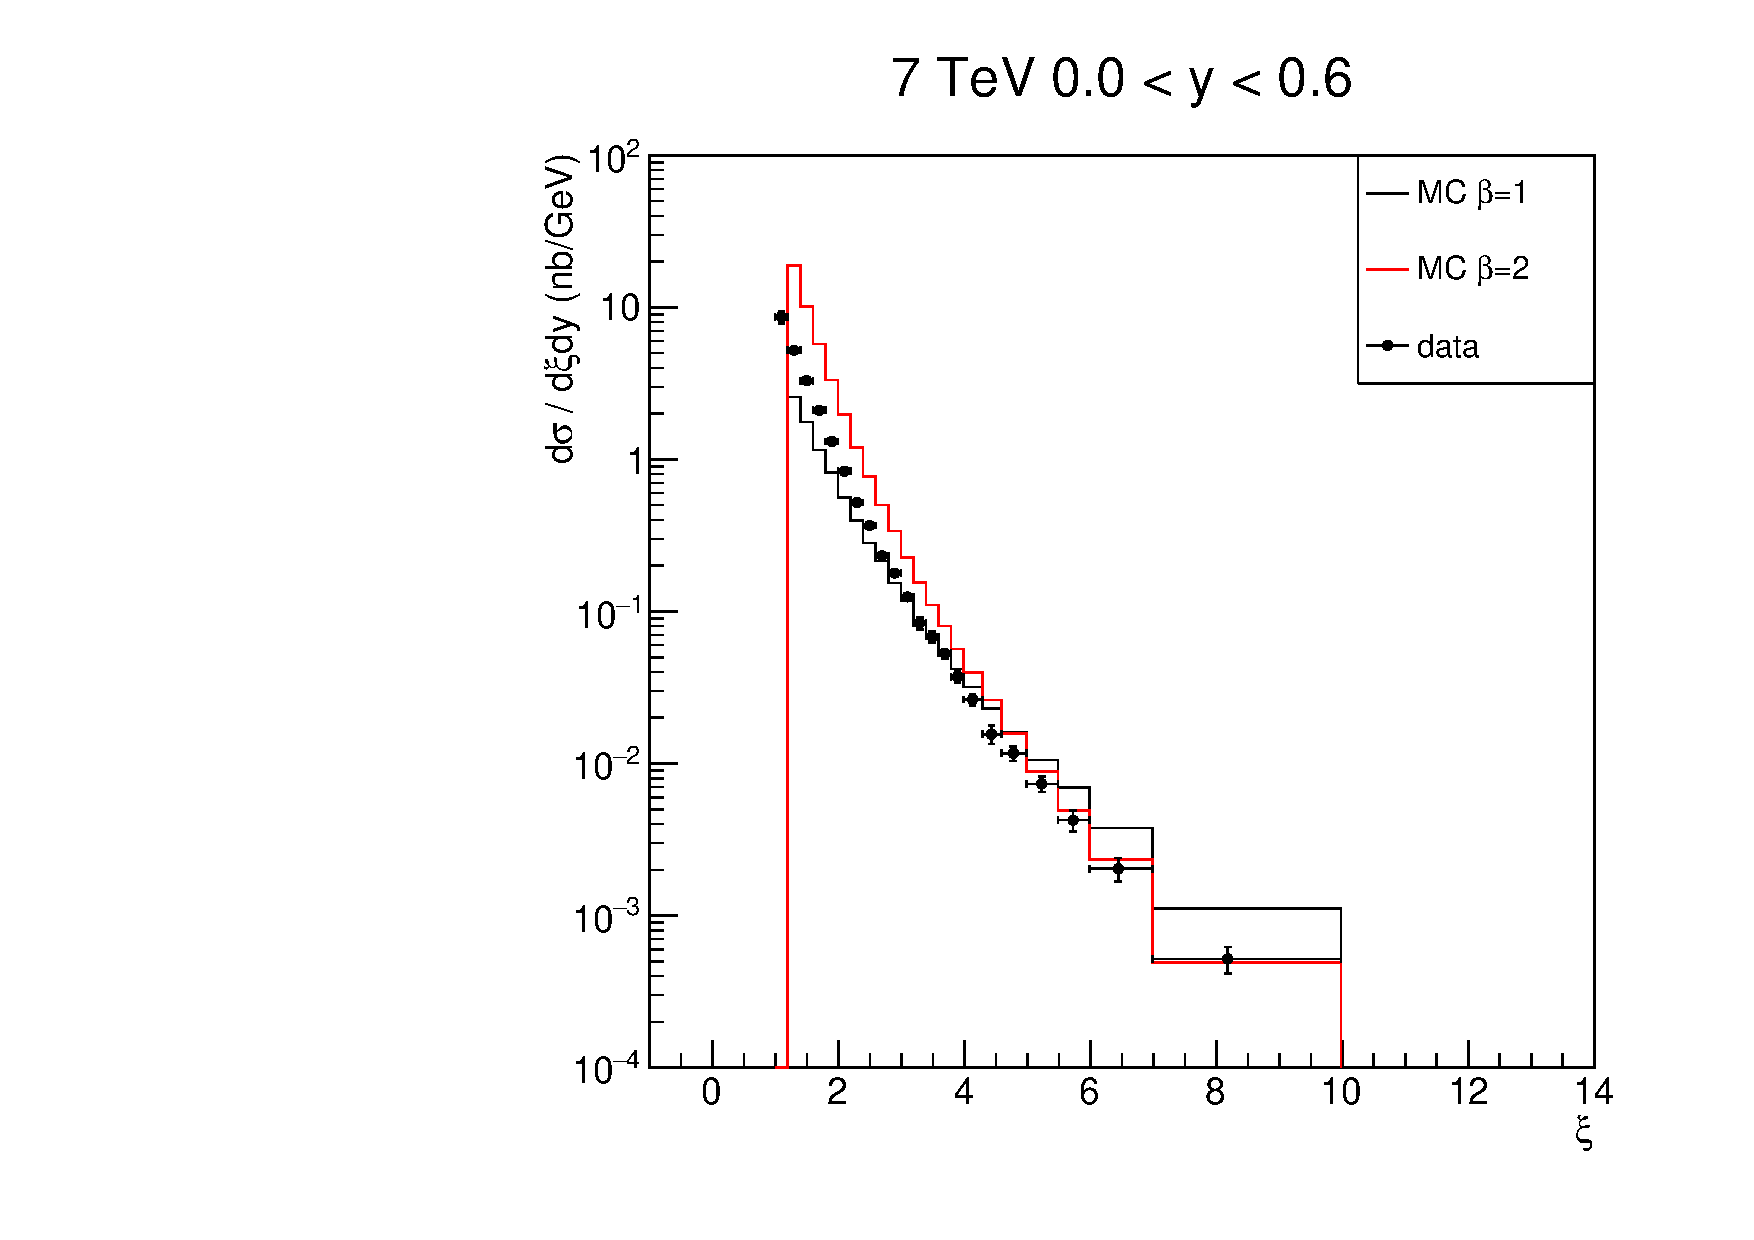
\includegraphics[width = 0.4\textwidth]{xi_7_y1.pdf}
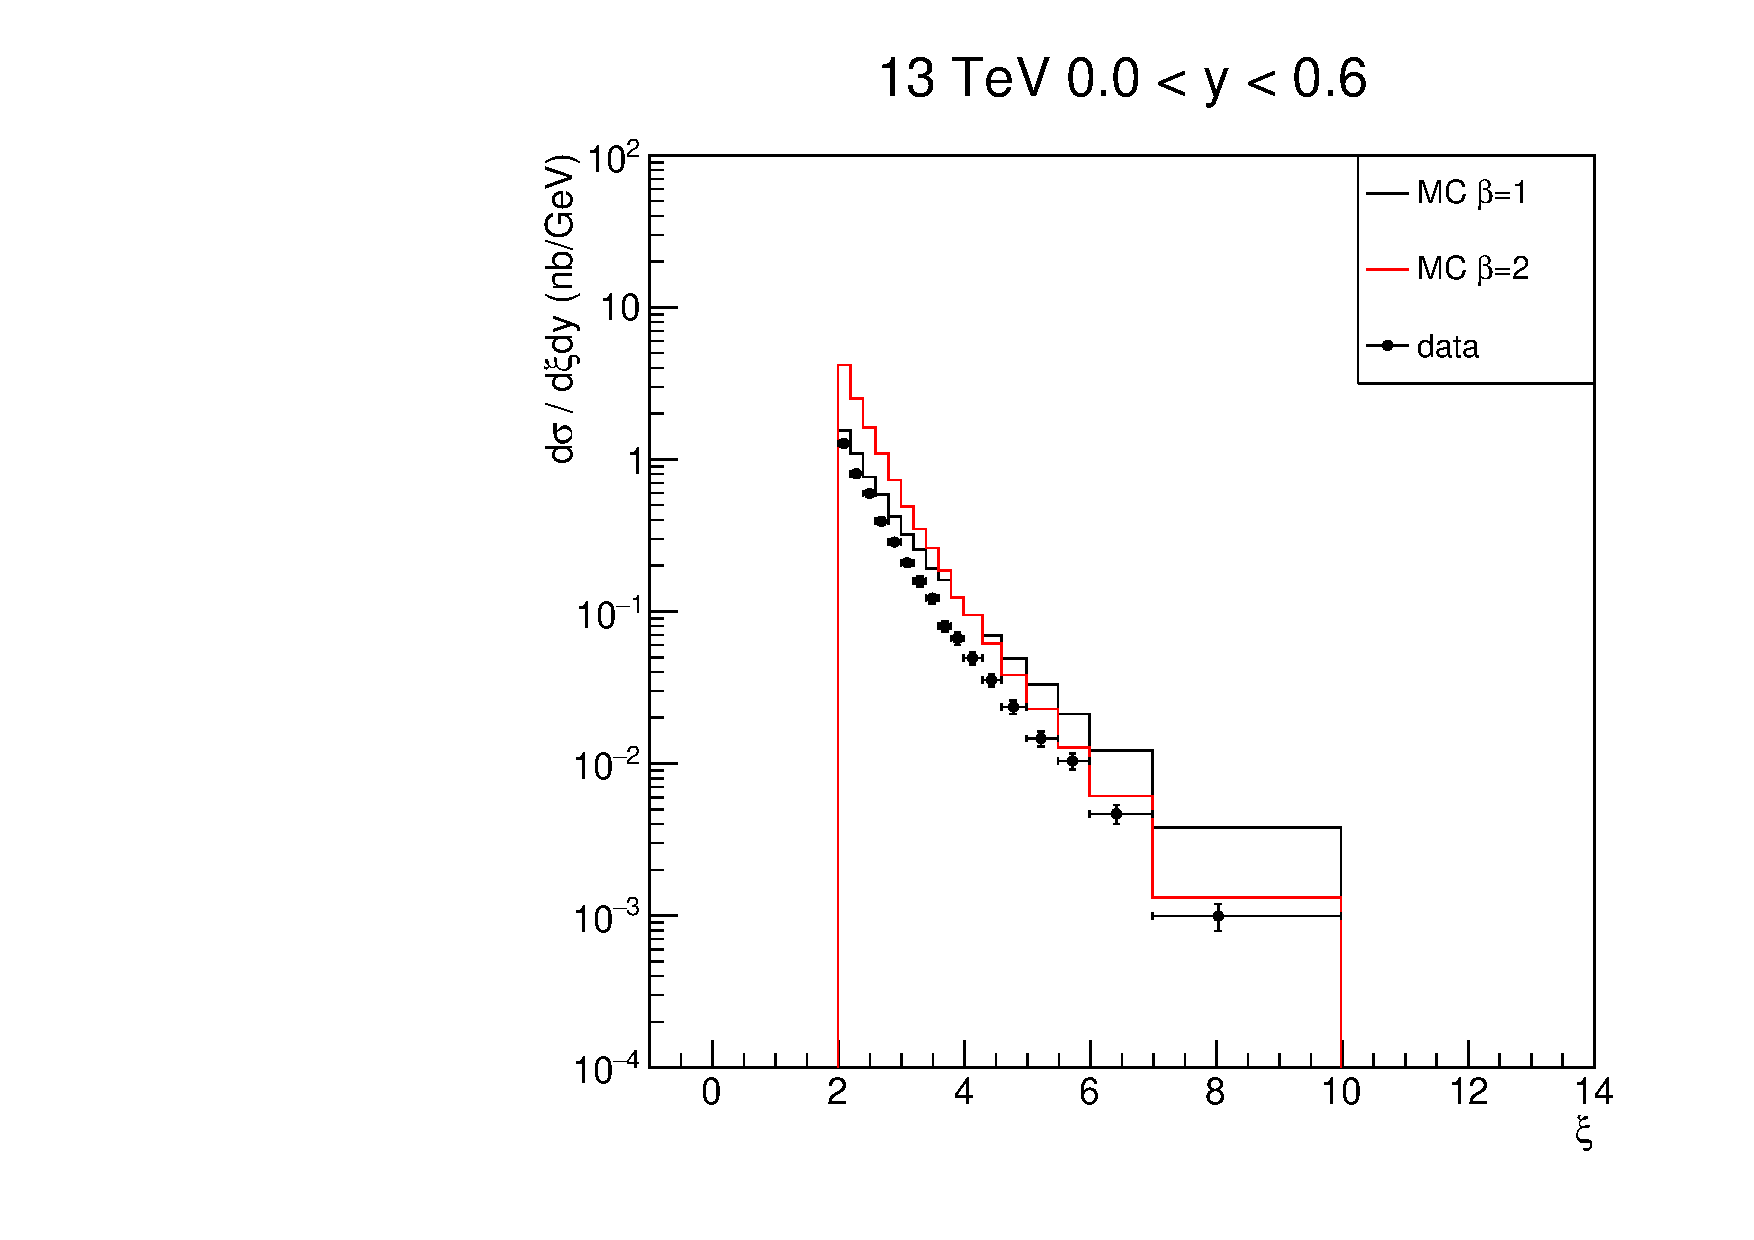
\includegraphics[width = 0.4\textwidth]{xi_13_y1.pdf}

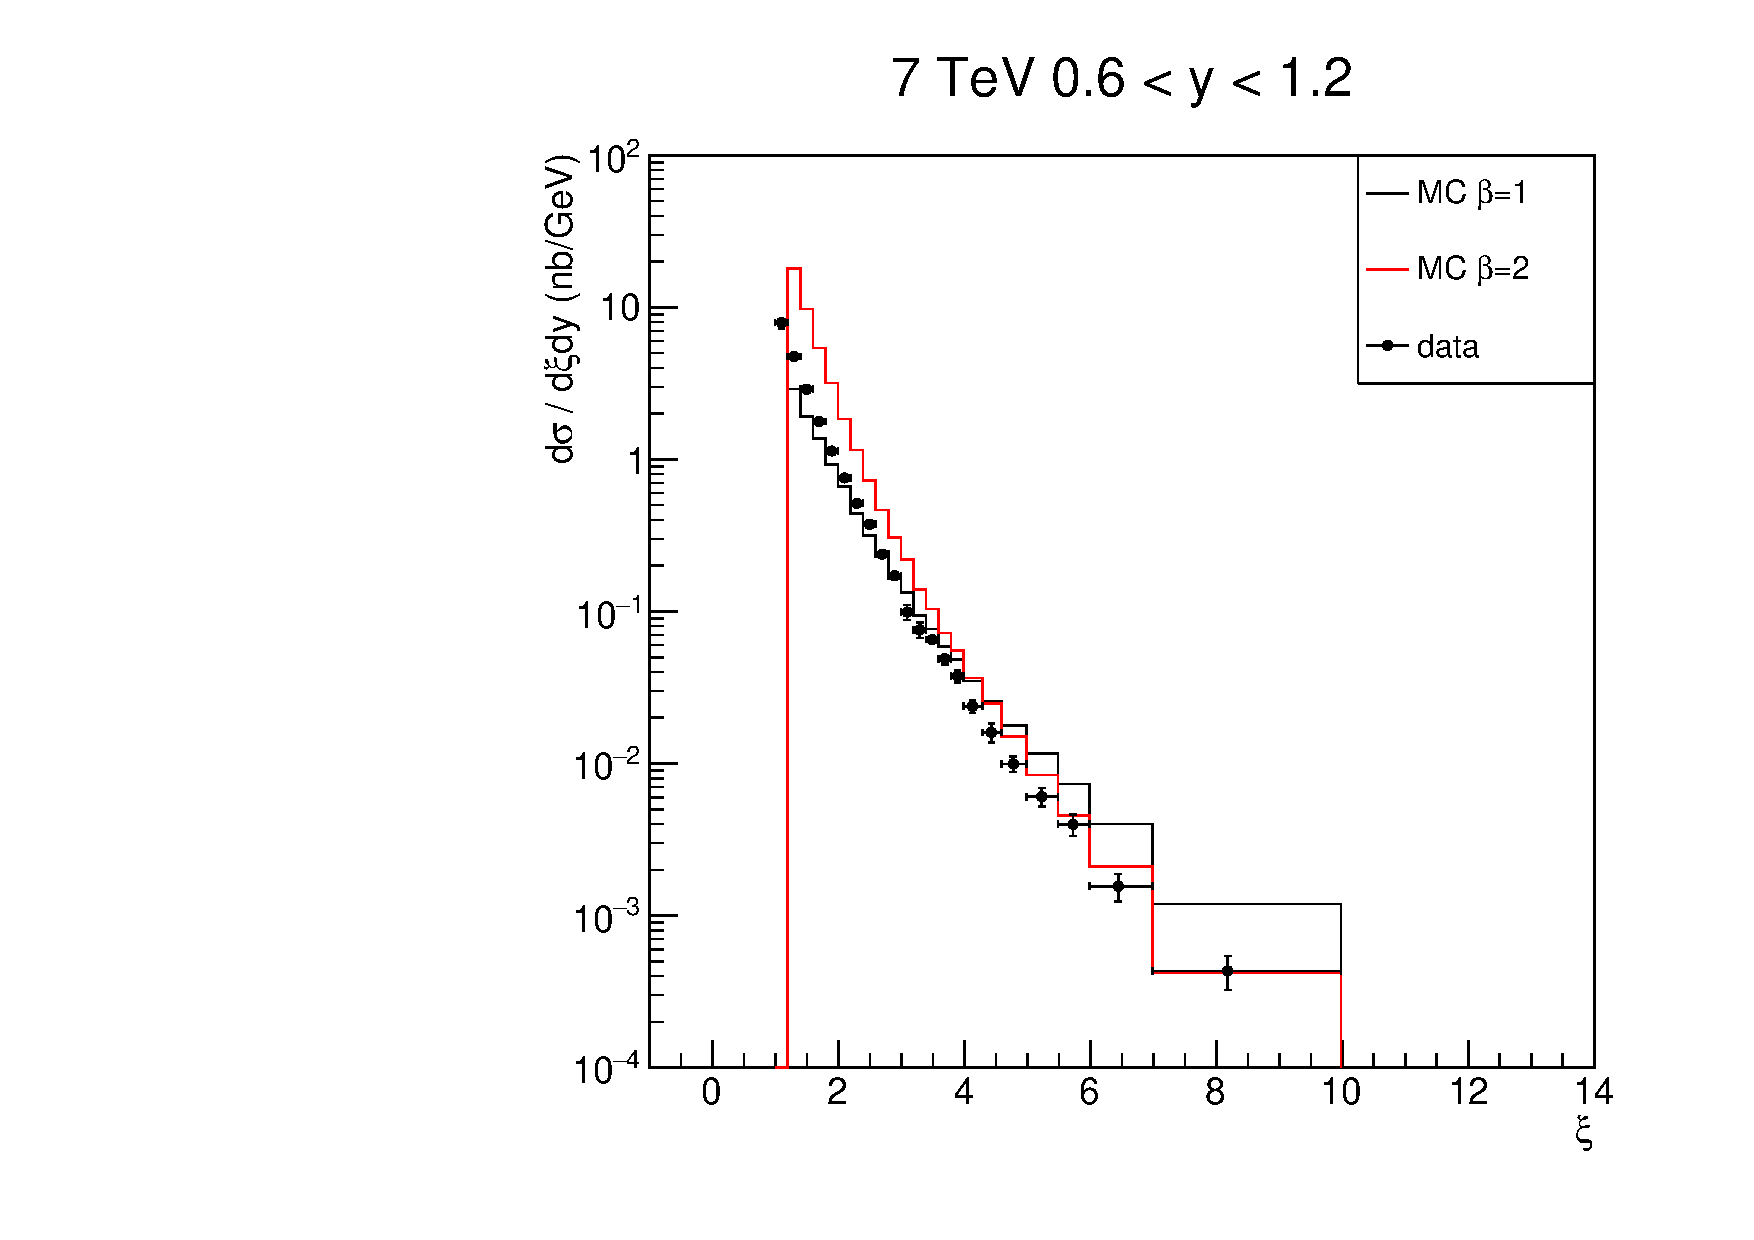
\includegraphics[width = 0.4\textwidth]{xi_7_y2.pdf}
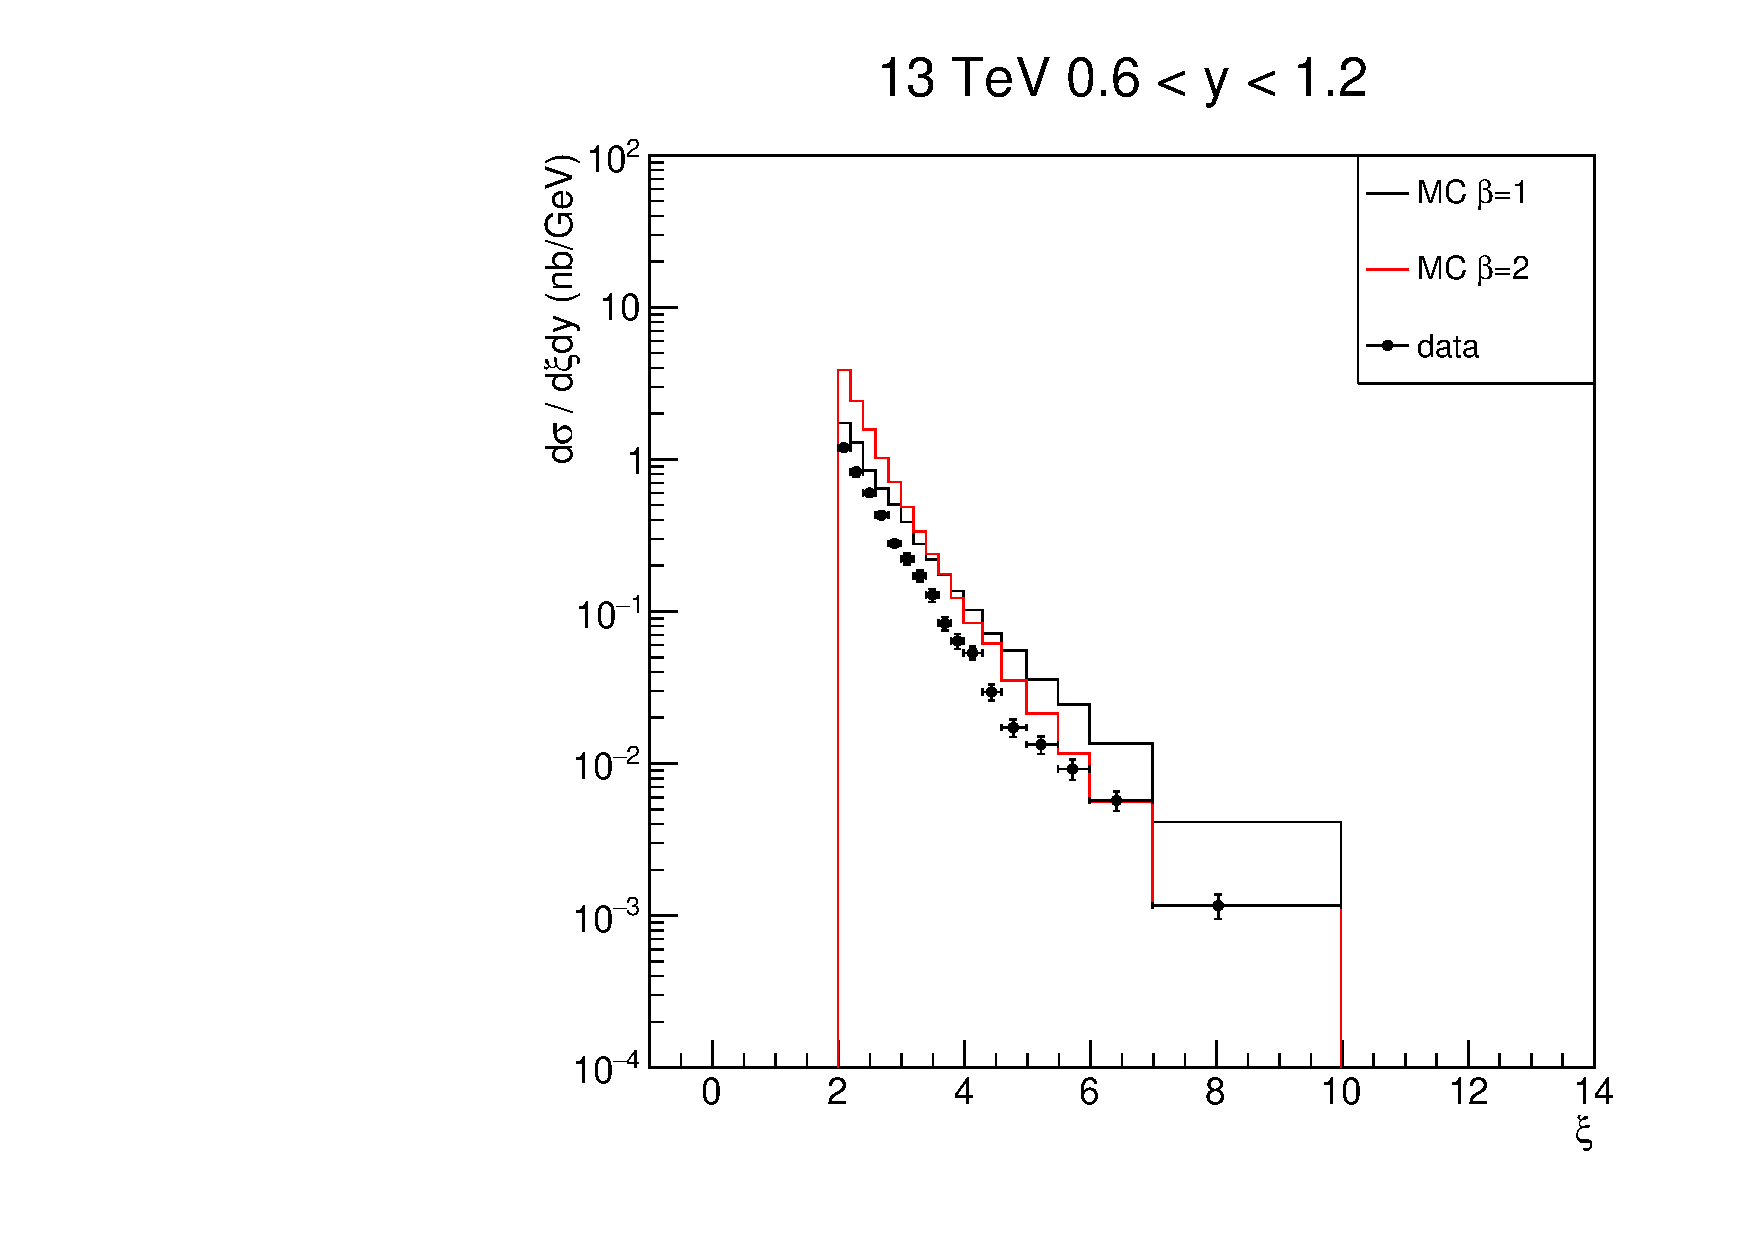
\includegraphics[width = 0.4\textwidth]{xi_13_y2.pdf}
\caption{Comparison between MC $\xi$ distribution and data points in the first three $y$ bins of the data, for 7 TeV (left) and 13 TeV (right). All histograms divided by total nr events and multiplied by same normalization factor. Data is not scaled.}\label{f:xi_comp_1}
\end{figure}

\clearpage

\begin{figure}[h!]
\centering
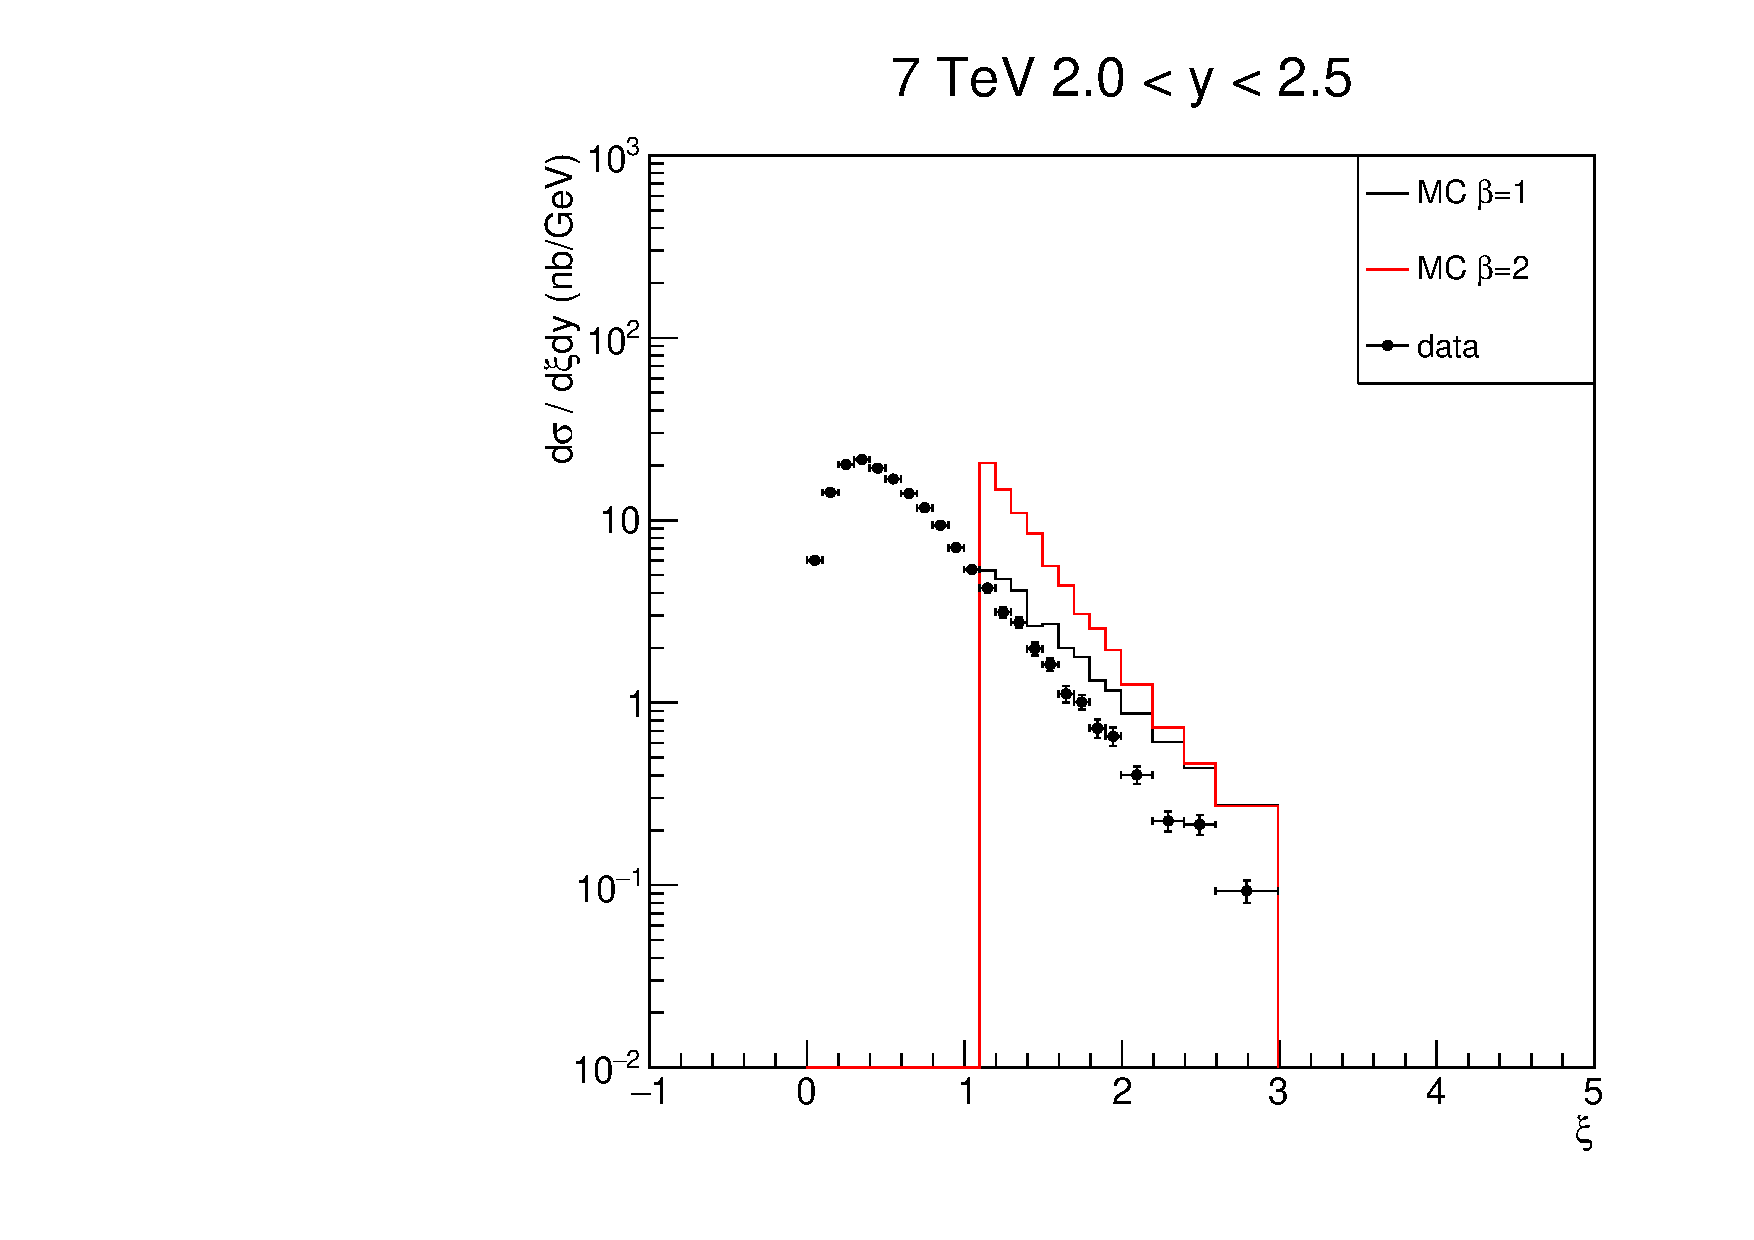
\includegraphics[width = 0.4\textwidth]{xi_7_y3.pdf}
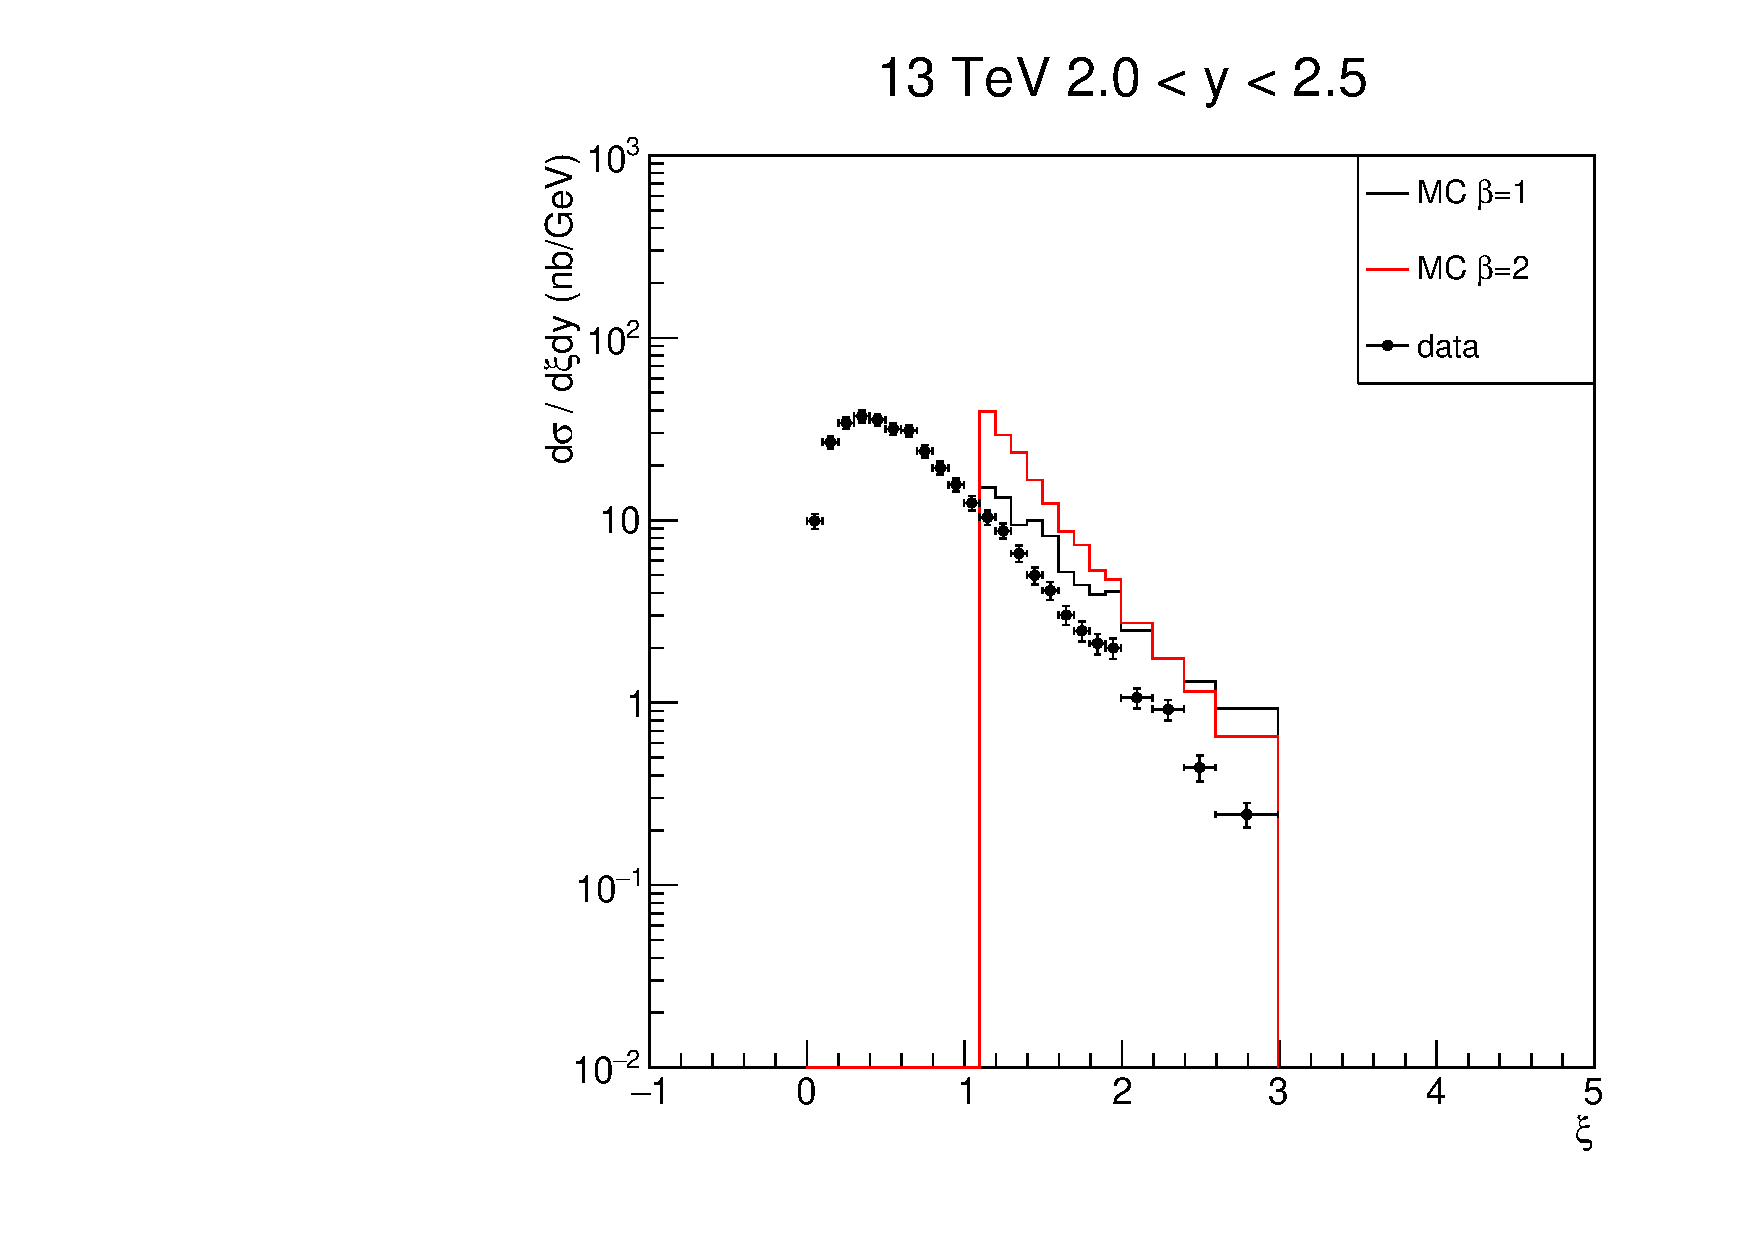
\includegraphics[width = 0.4\textwidth]{xi_13_y3.pdf}

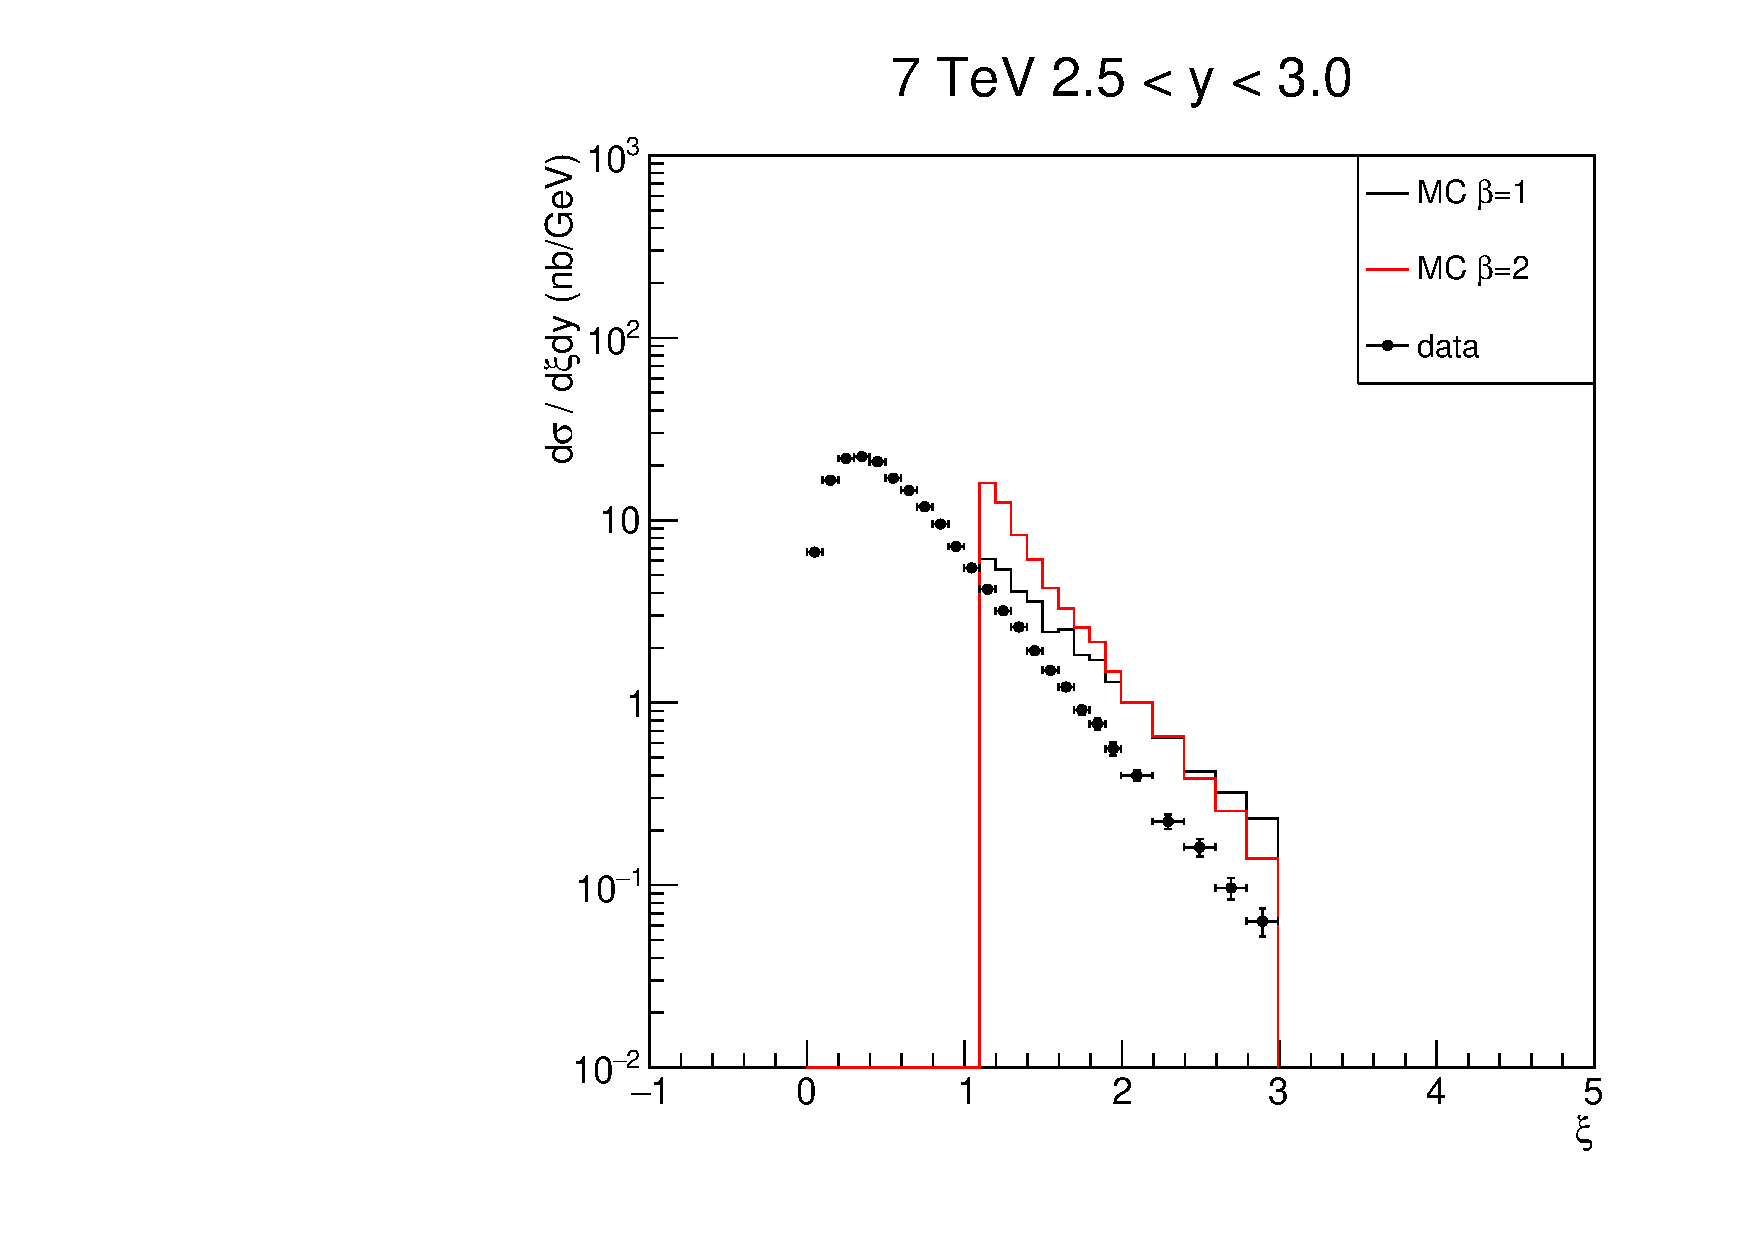
\includegraphics[width = 0.4\textwidth]{xi_7_y4.pdf}
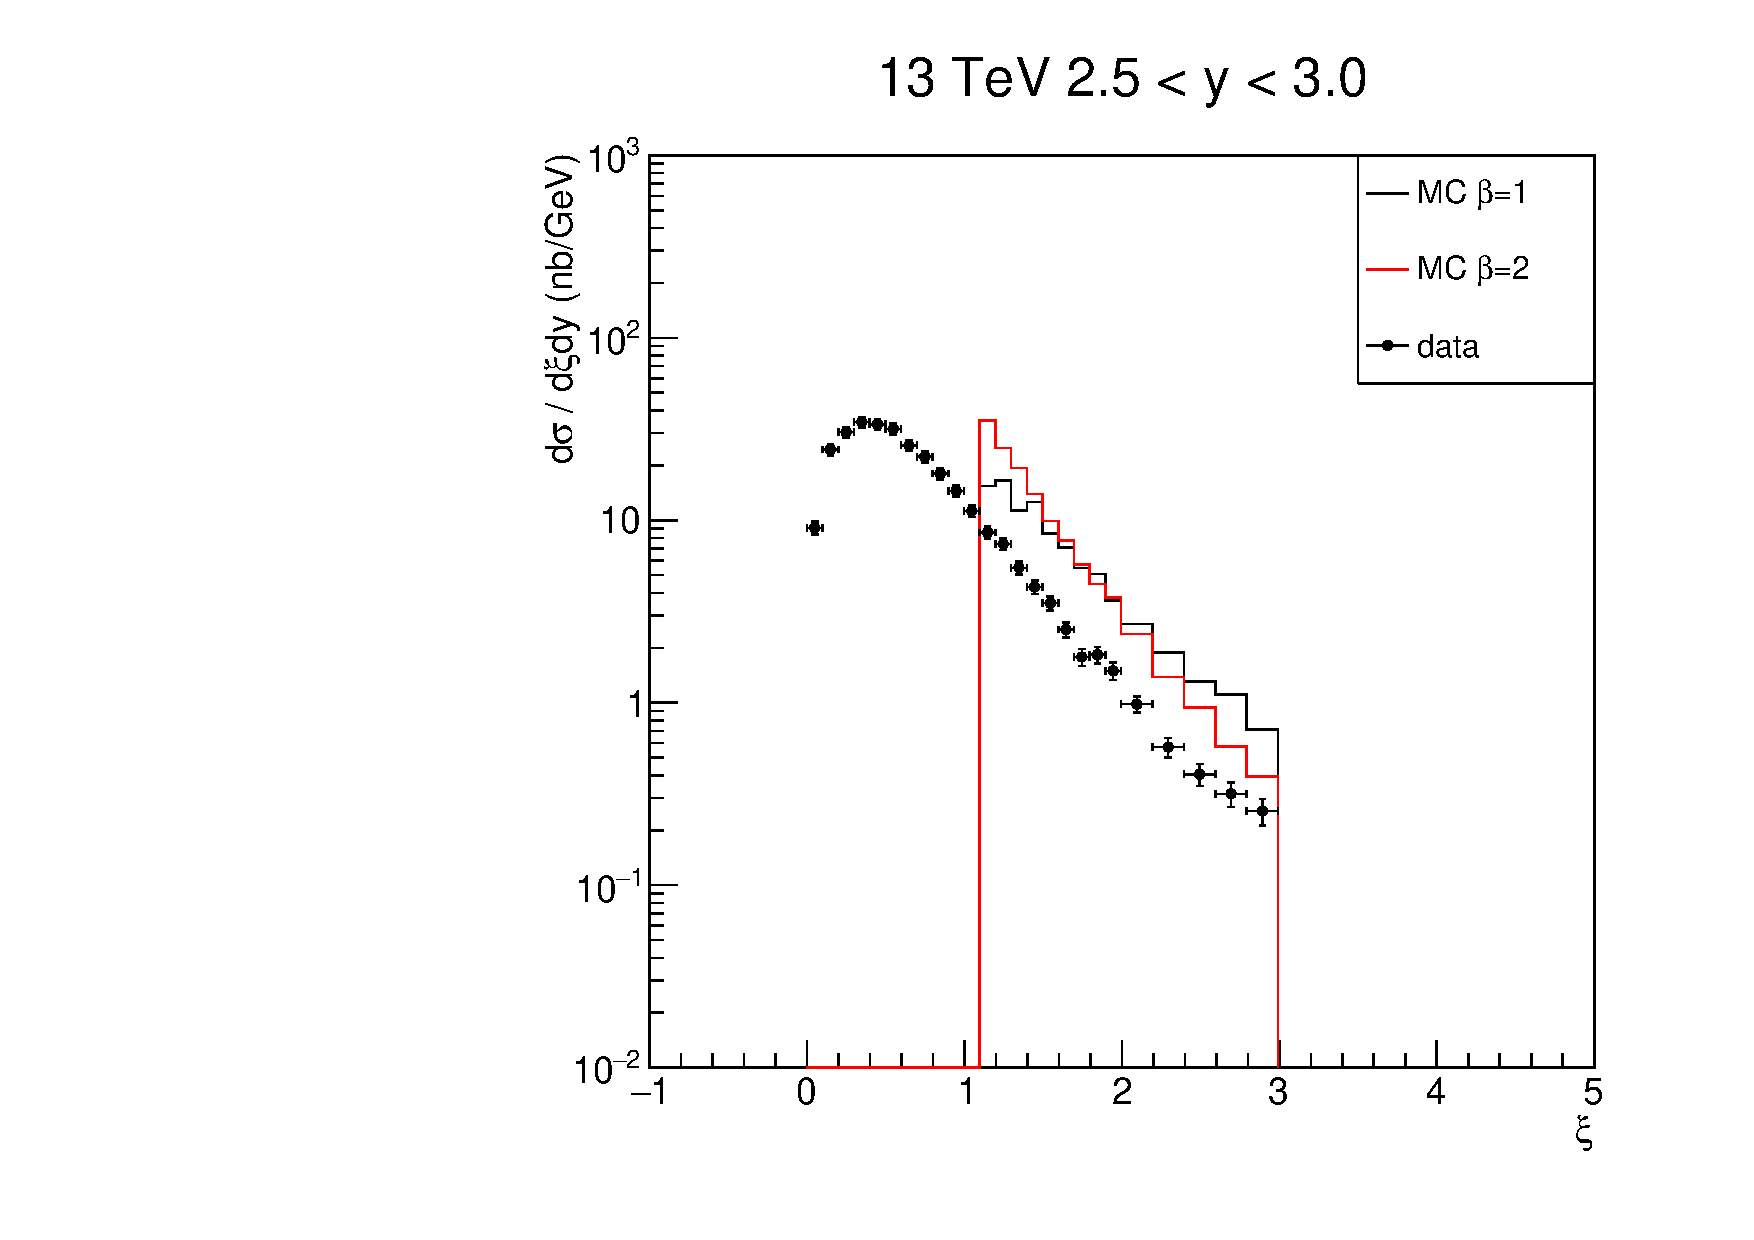
\includegraphics[width = 0.4\textwidth]{xi_13_y4.pdf}
\caption{Comparison between MC $\xi$ distribution and data points in the first three $y$ bins of the data, for 7 TeV (left) and 13 TeV (right). All histograms divided by total nr events and multiplied by same normalization factor. Data is not scaled.}\label{f:xi_comp_2}
\end{figure}

\clearpage

\begin{figure}[h!]
\centering
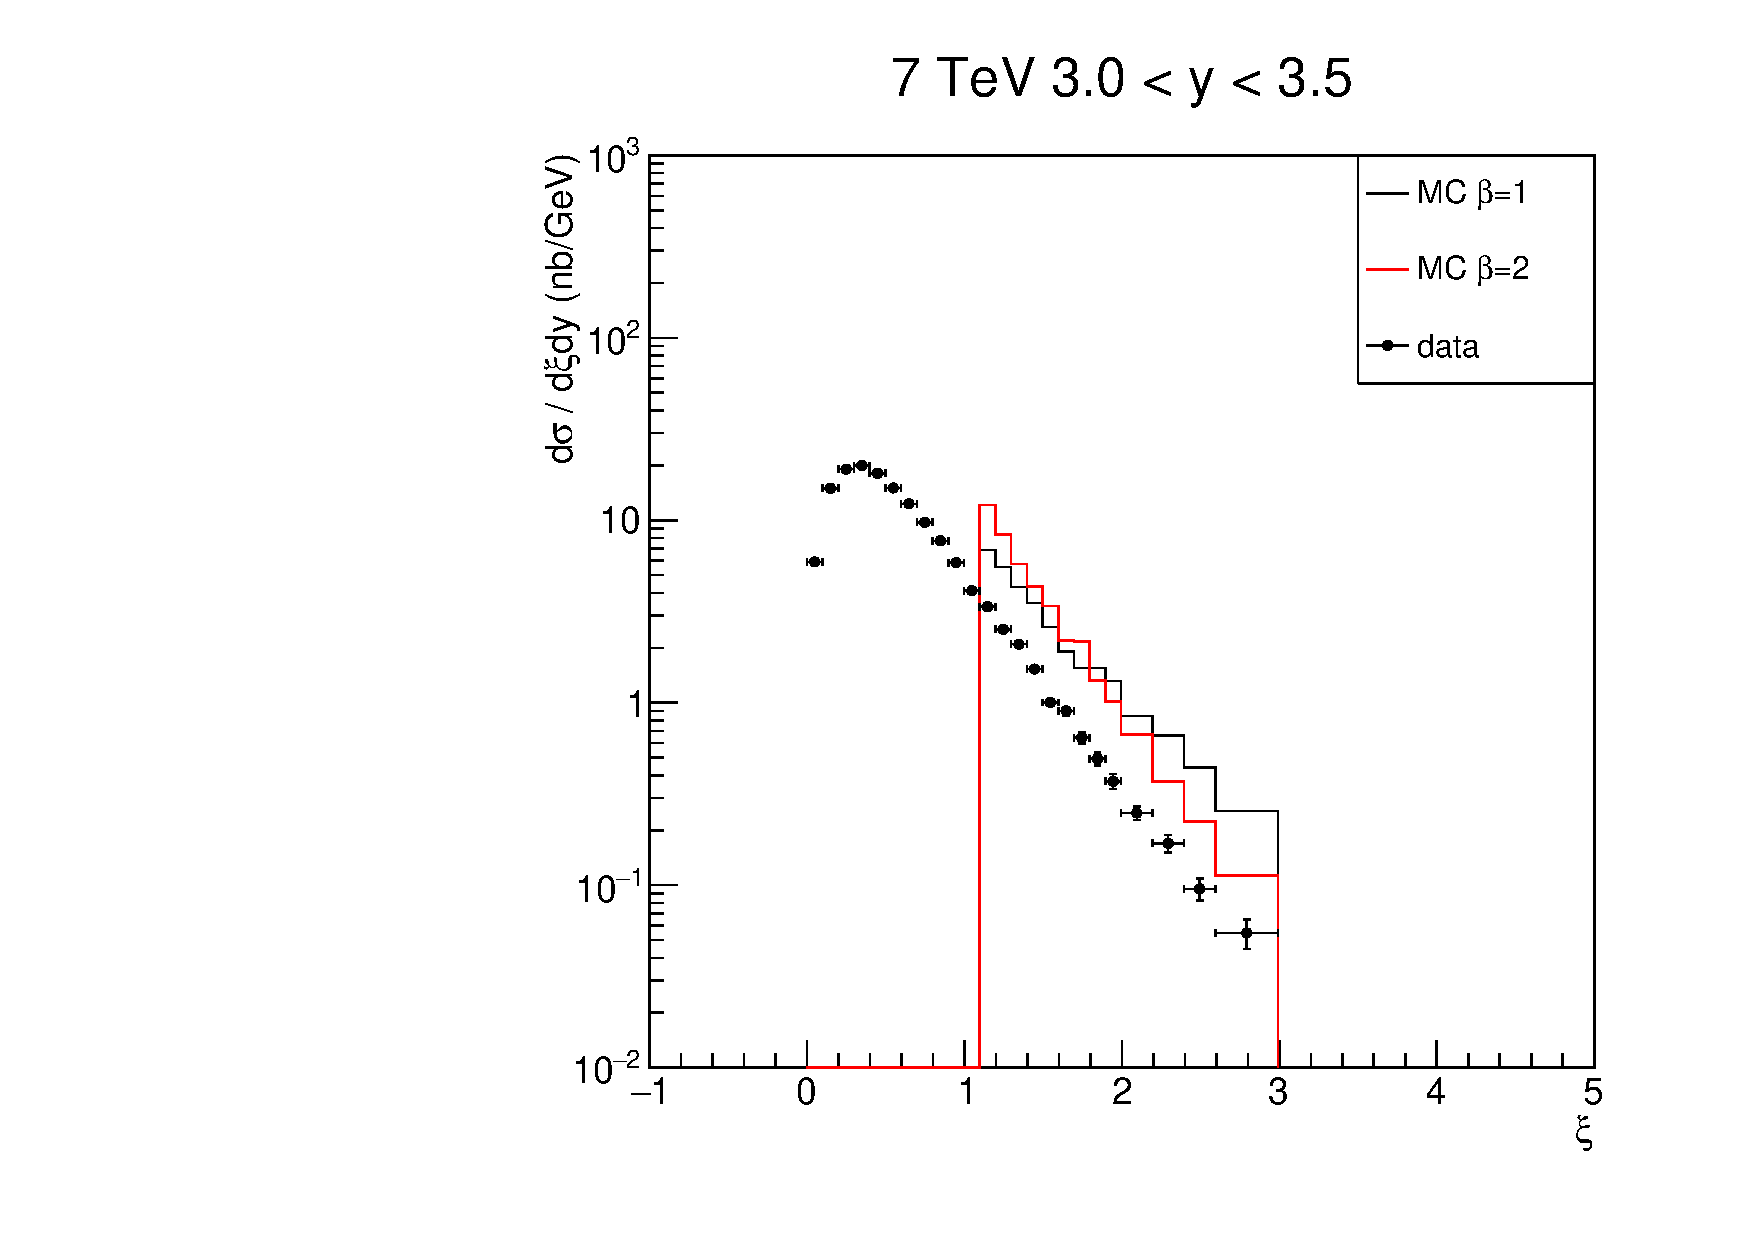
\includegraphics[width = 0.4\textwidth]{xi_7_y5.pdf}
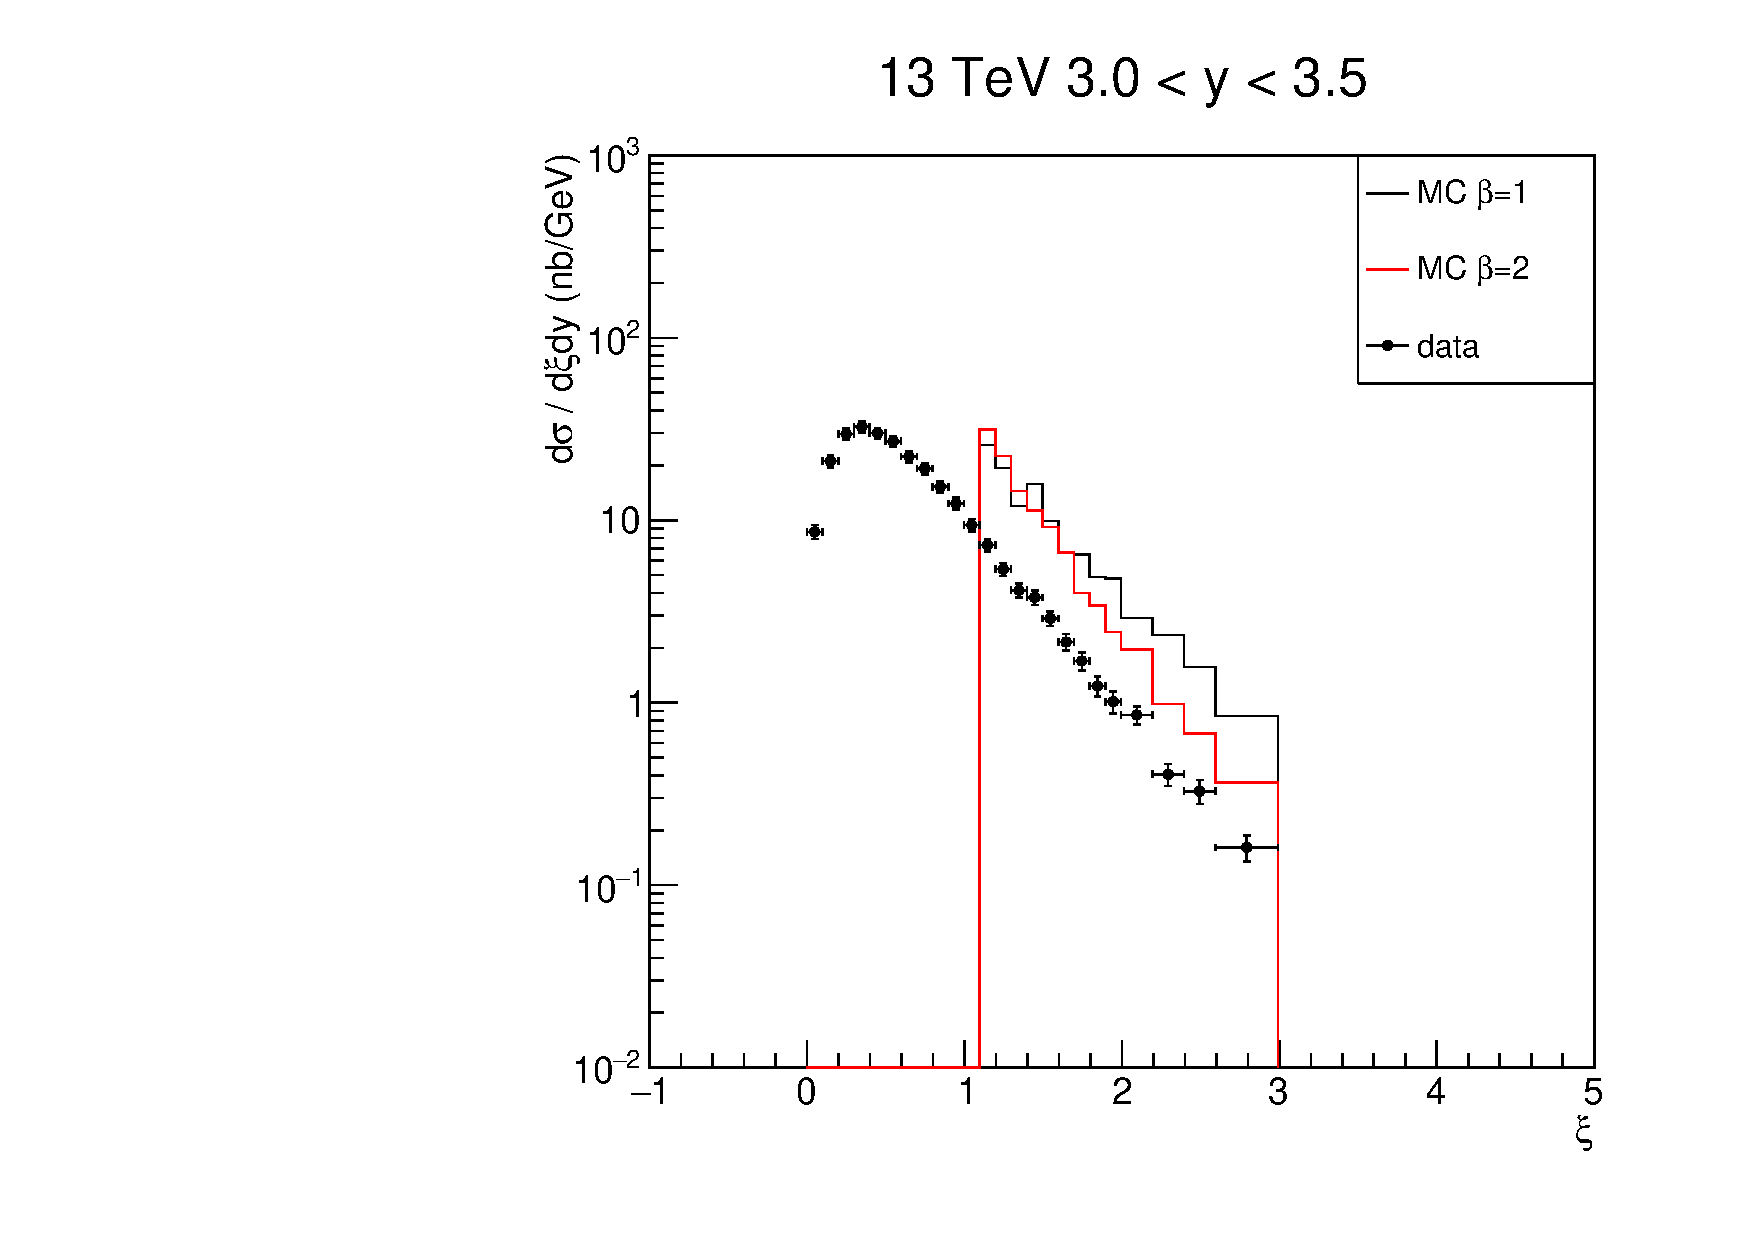
\includegraphics[width = 0.4\textwidth]{xi_13_y5.pdf}

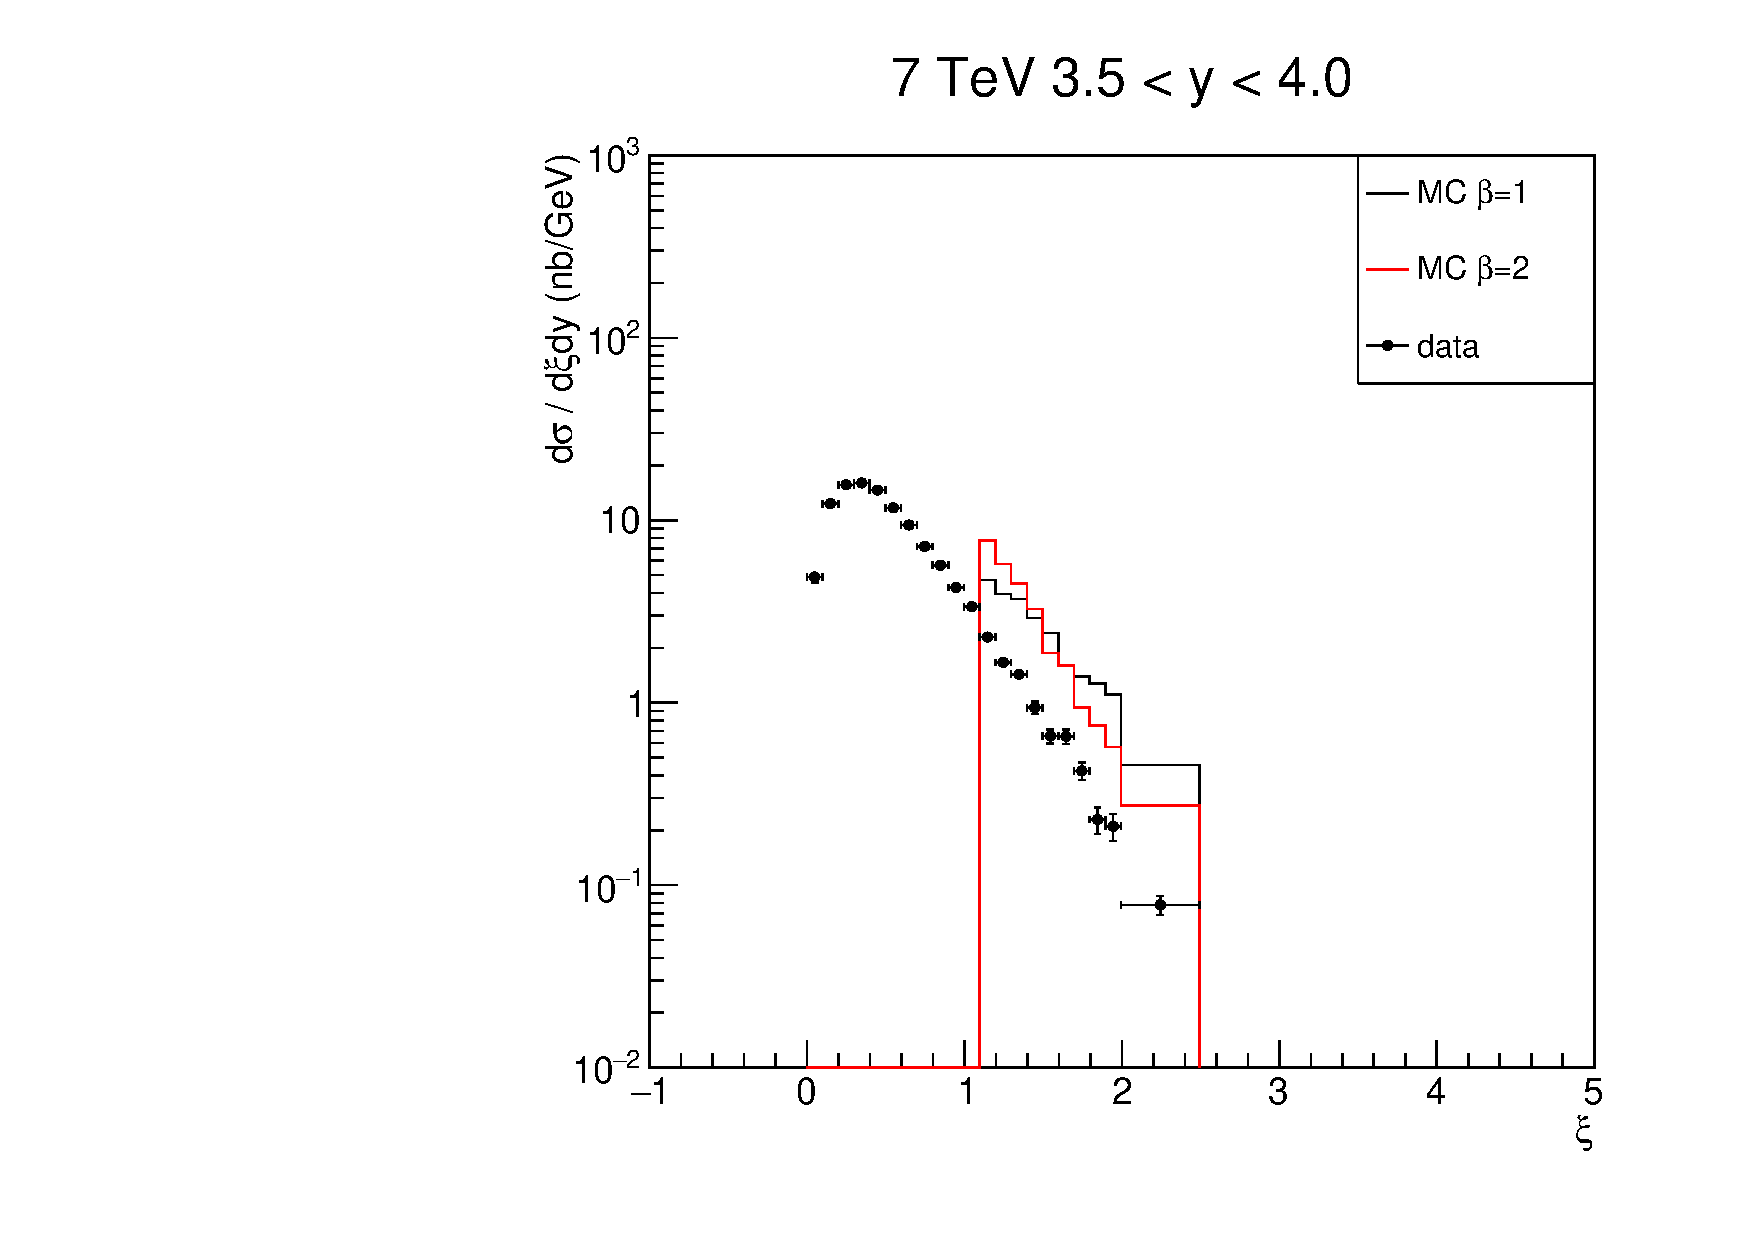
\includegraphics[width = 0.4\textwidth]{xi_7_y6.pdf}
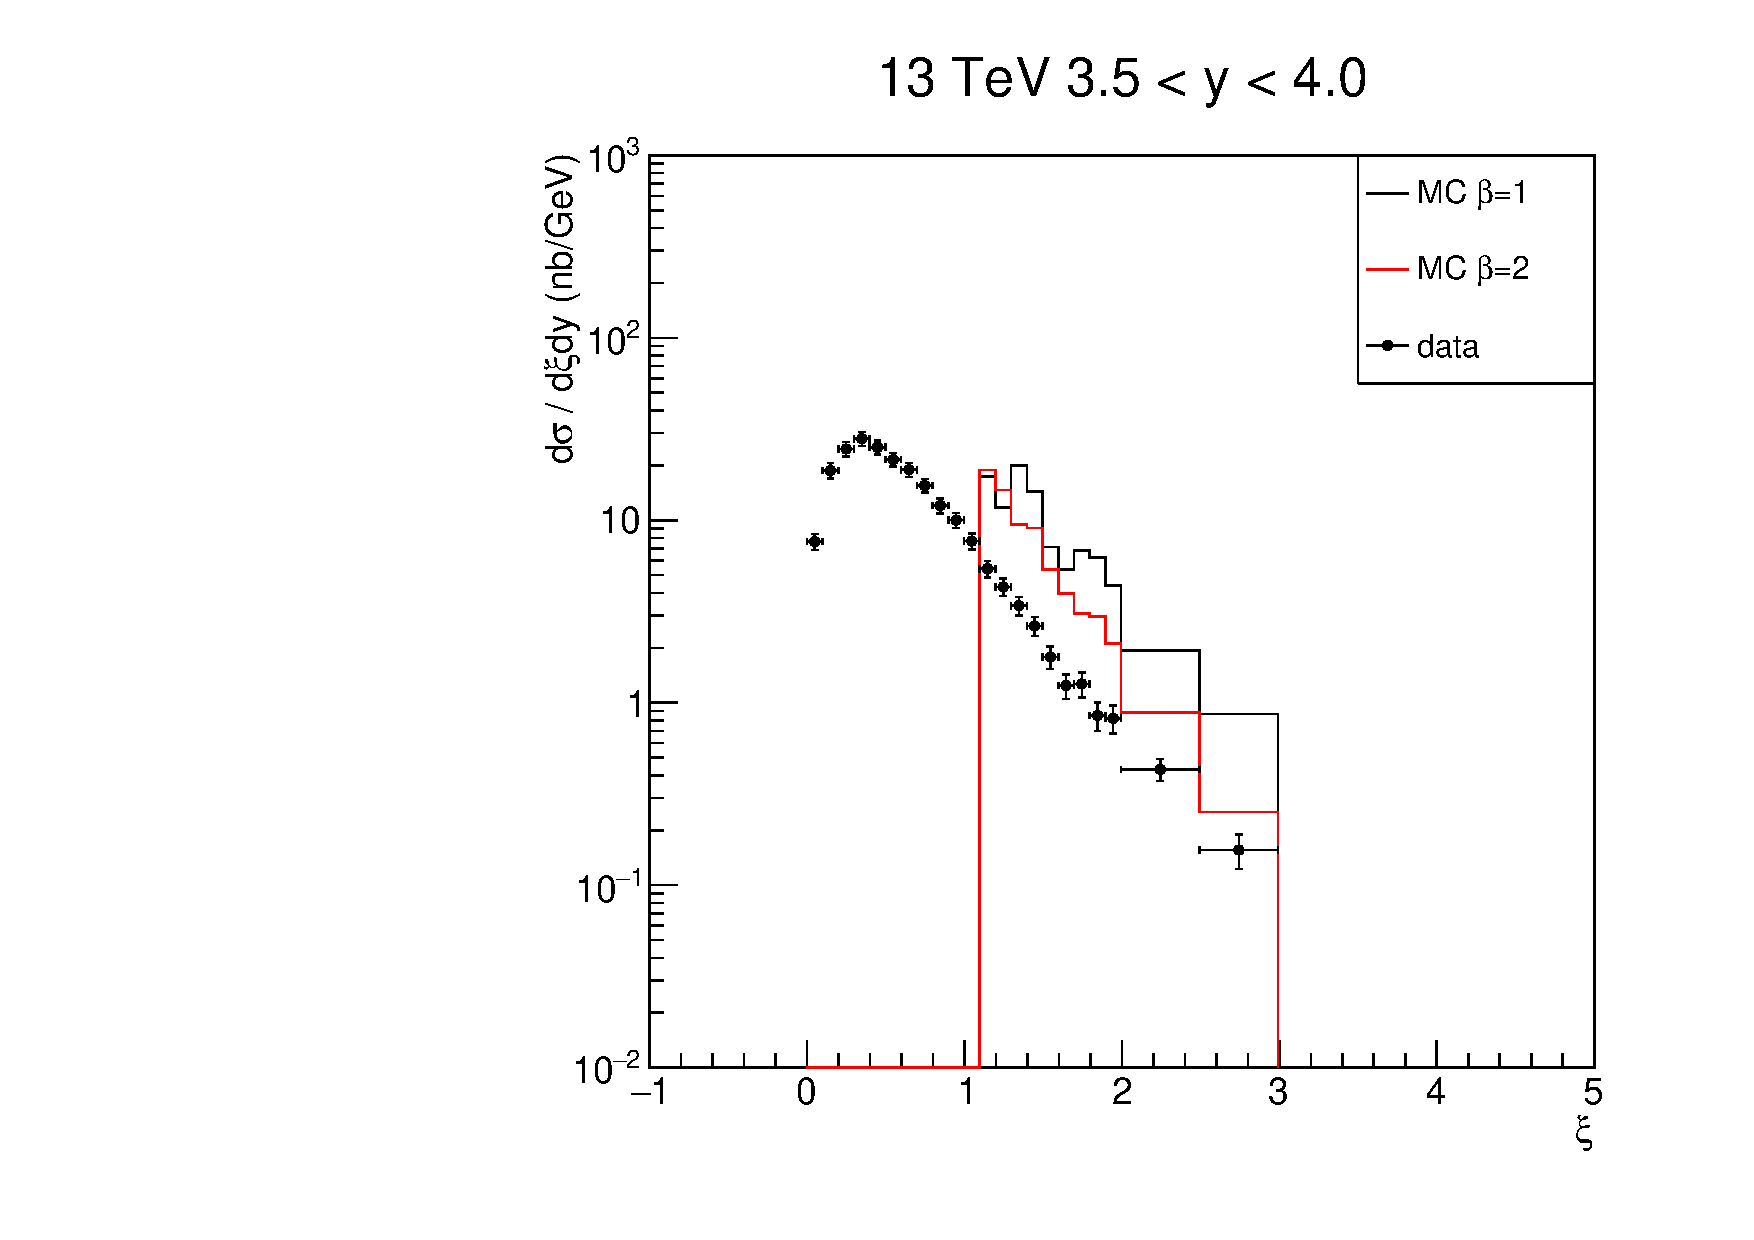
\includegraphics[width = 0.4\textwidth]{xi_13_y6.pdf}

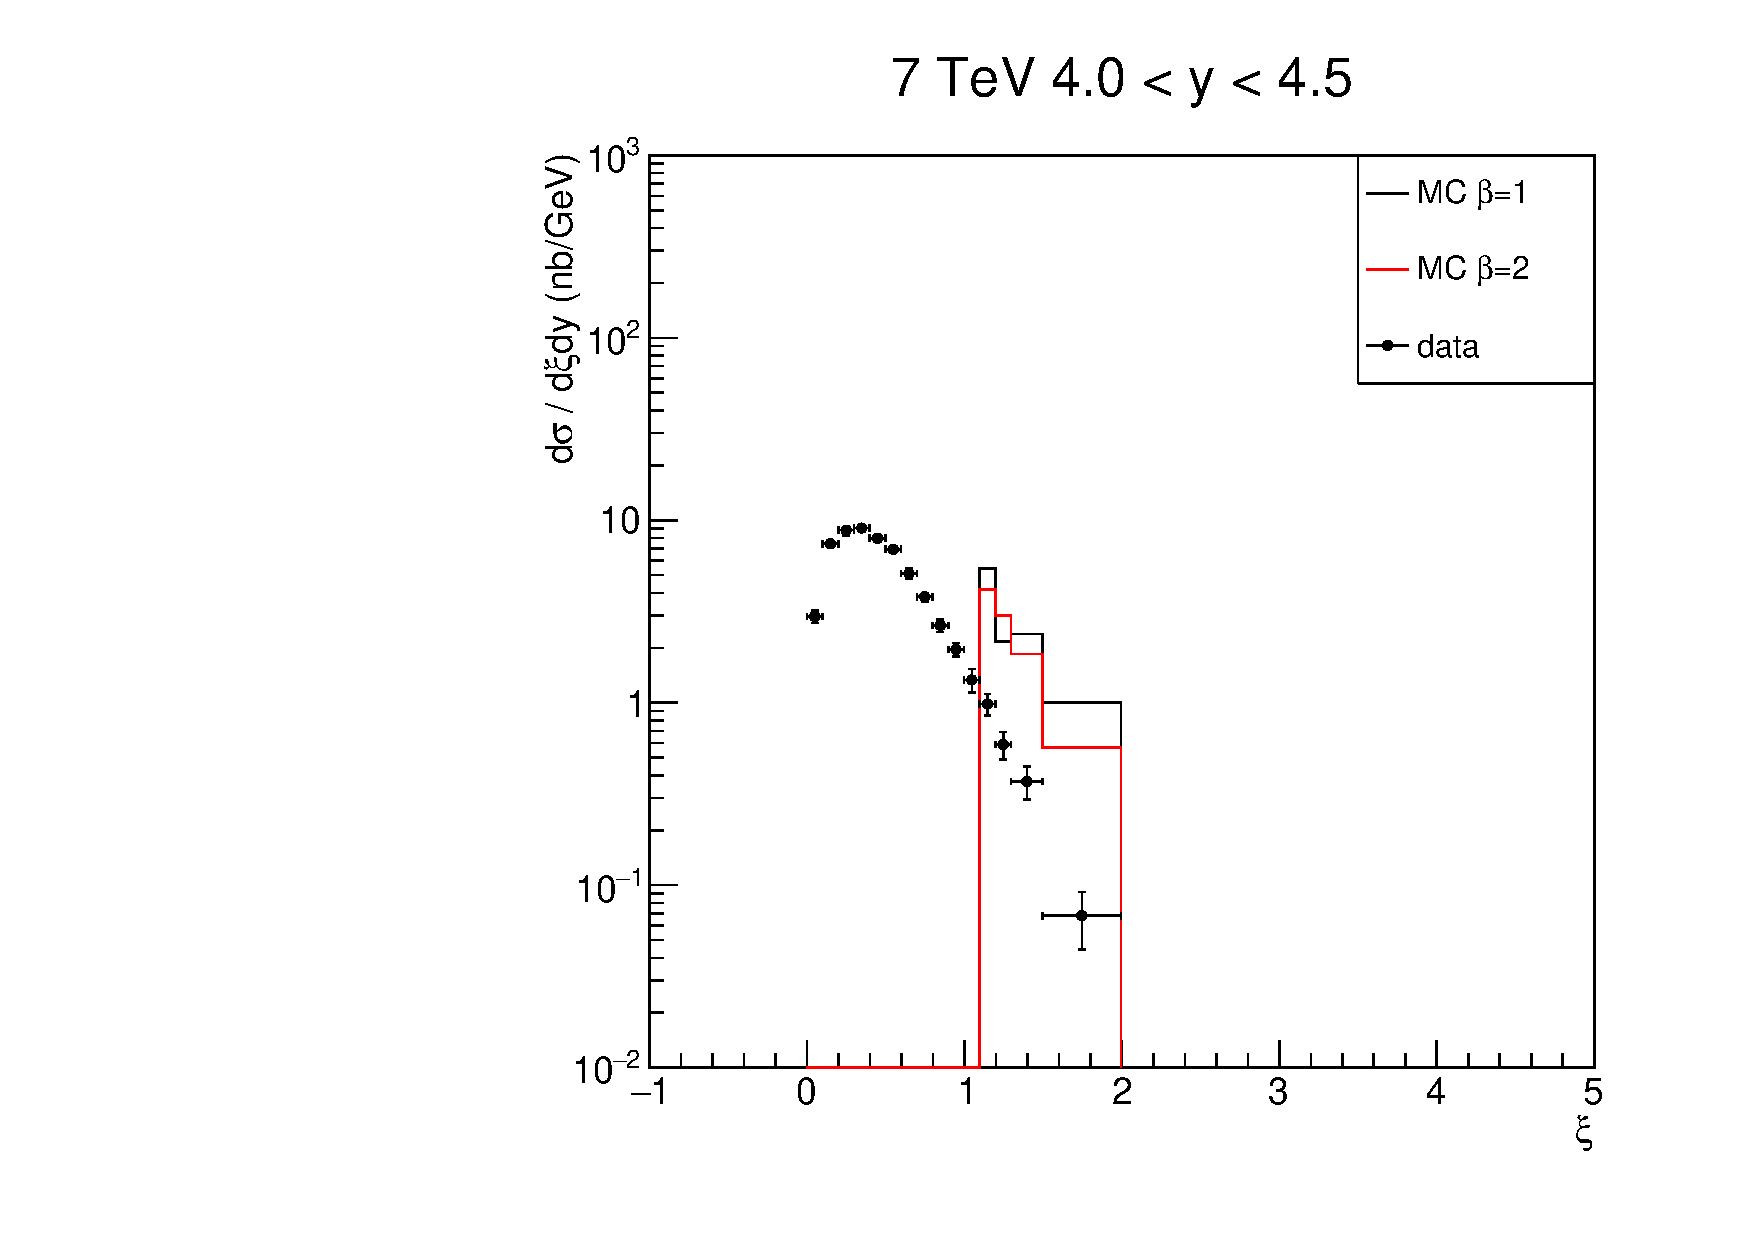
\includegraphics[width = 0.4\textwidth]{xi_7_y7.pdf}
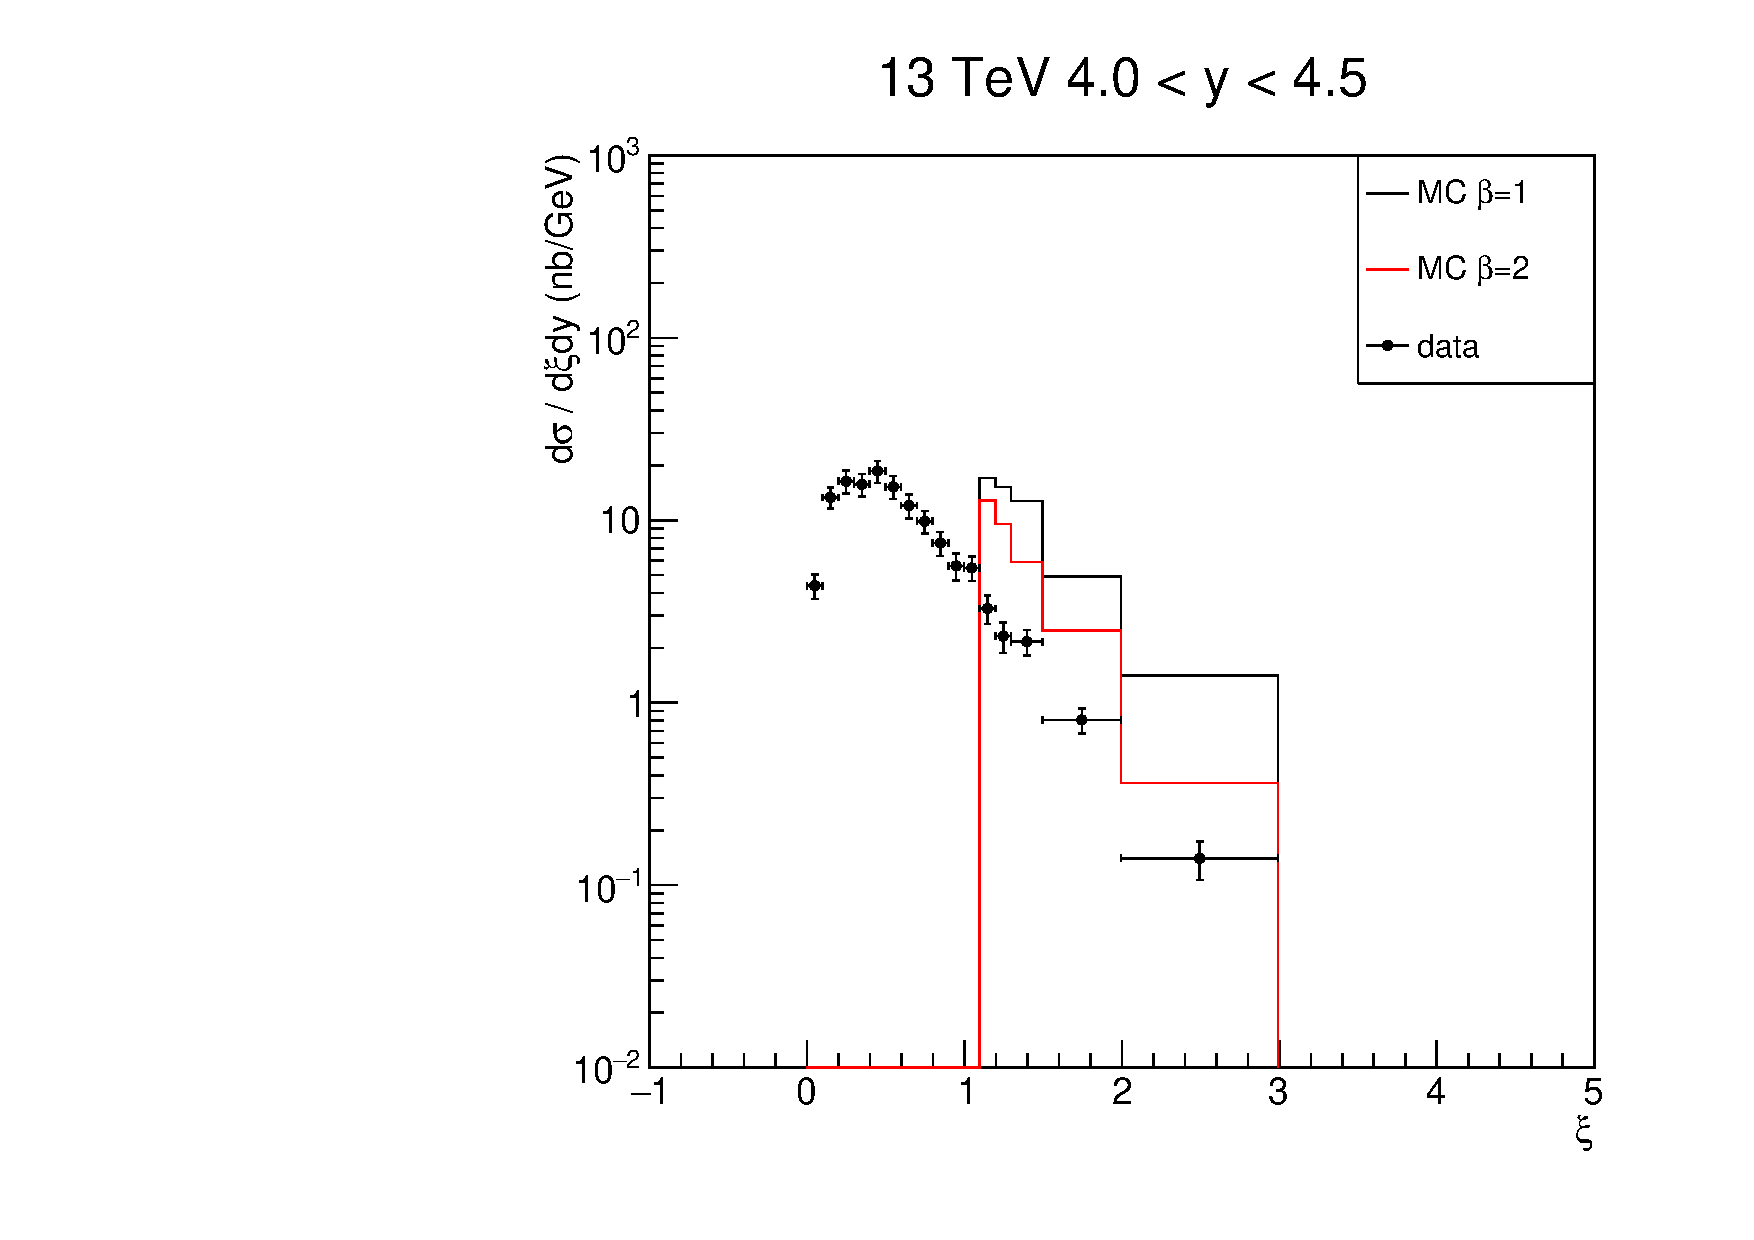
\includegraphics[width = 0.4\textwidth]{xi_13_y7.pdf}
\caption{Comparison between MC $\xi$ distribution and data points in the last three $y$ bins of the data, for 7 TeV (left) and 13 TeV (right). All histograms divided by total nr events and multiplied by same normalization factor. Data is not scaled.}\label{f:xi_comp_3}
\end{figure}

\clearpage

\begin{figure}[h!]
\centering
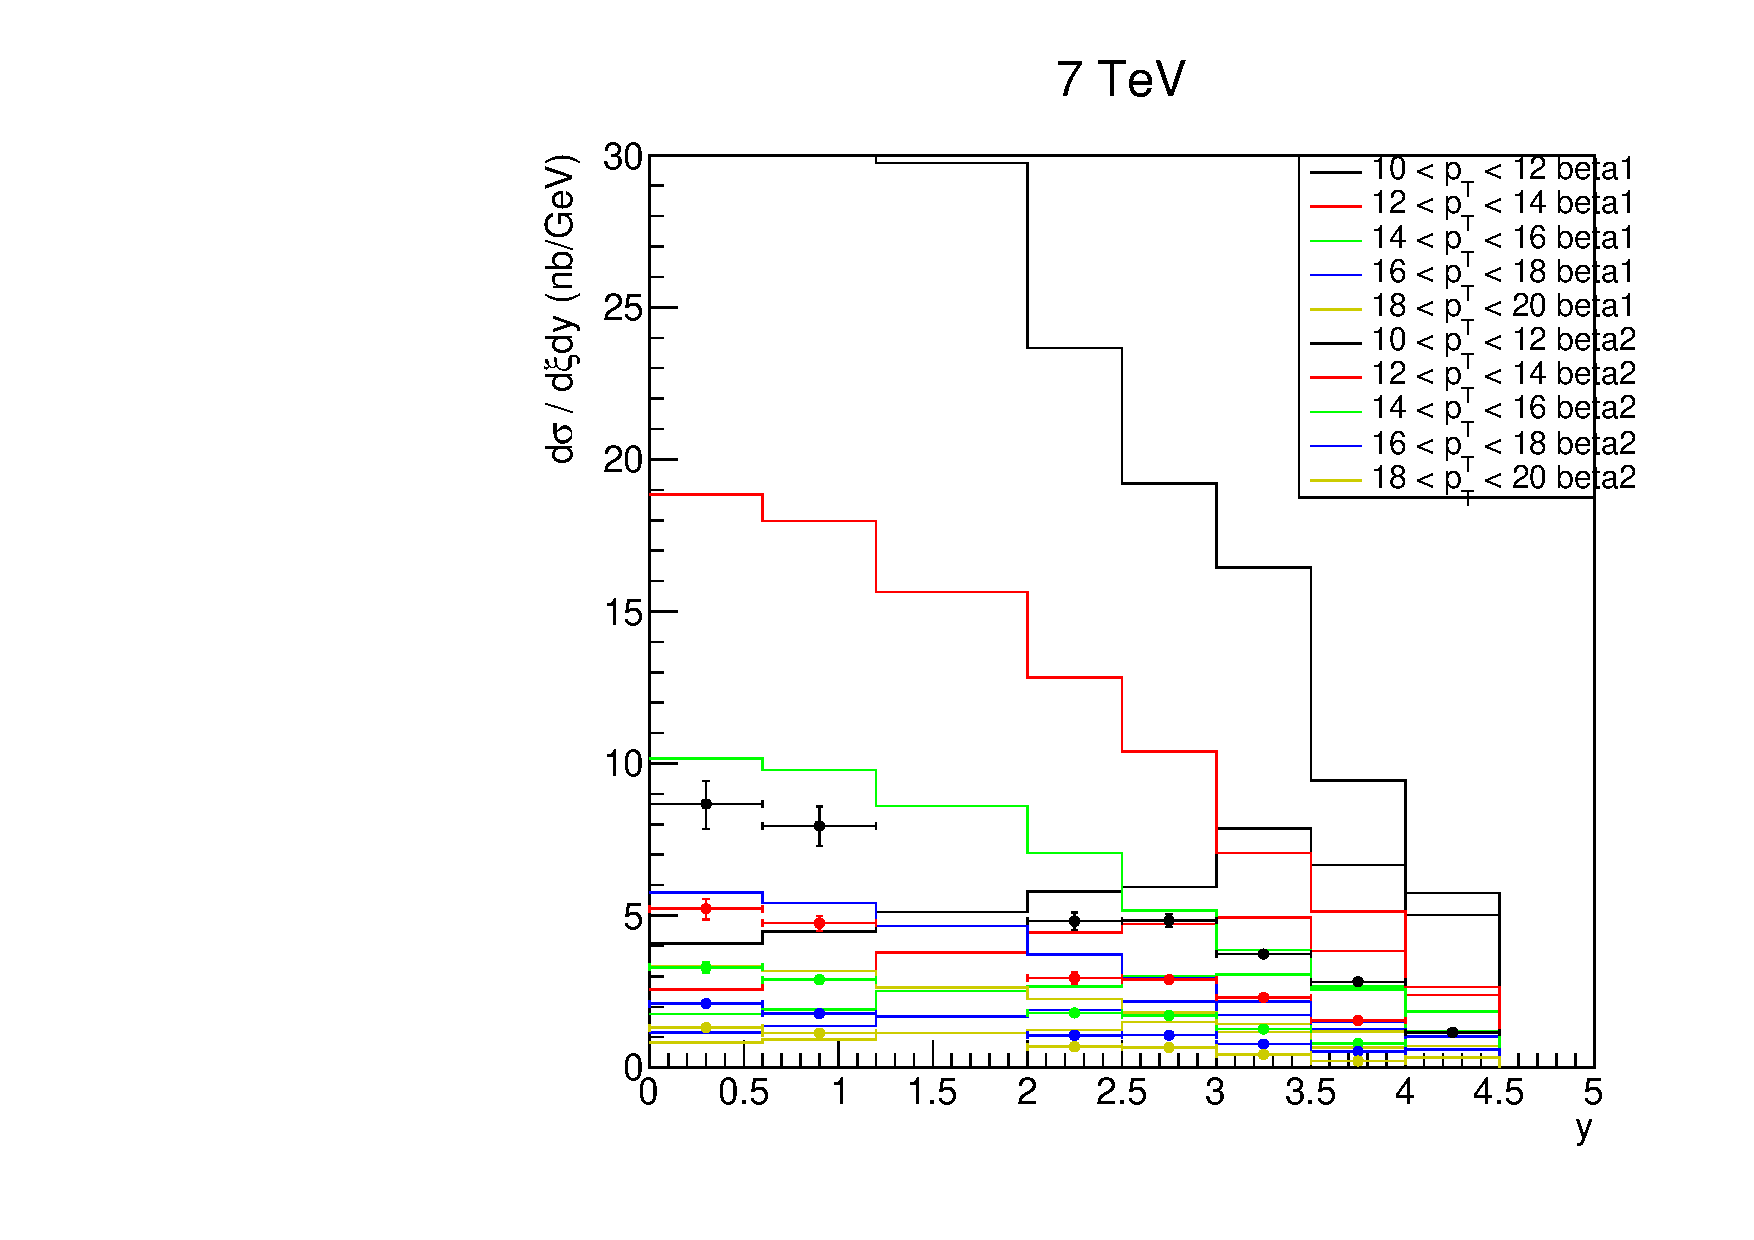
\includegraphics[width = 0.4\textwidth]{y_dist_7.pdf}
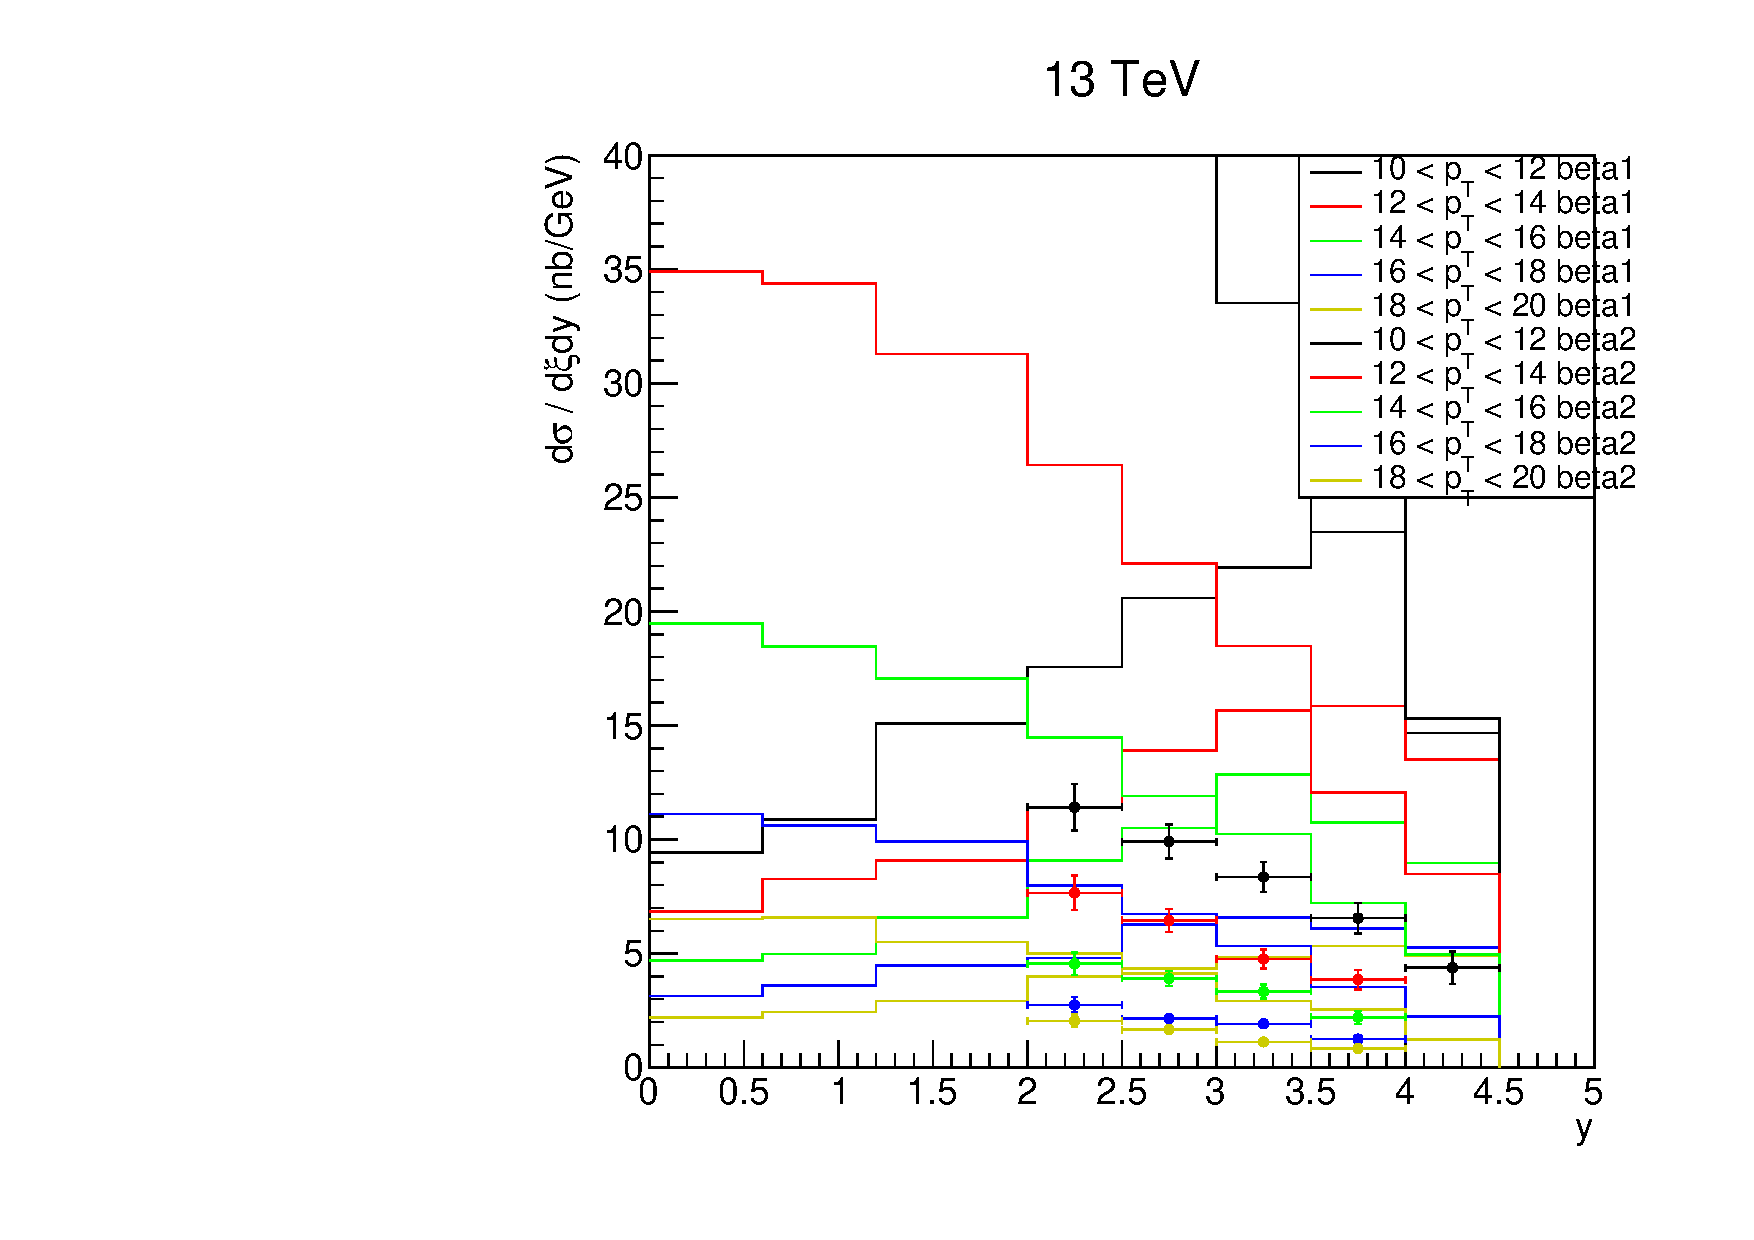
\includegraphics[width = 0.4\textwidth]{y_dist_13.pdf}

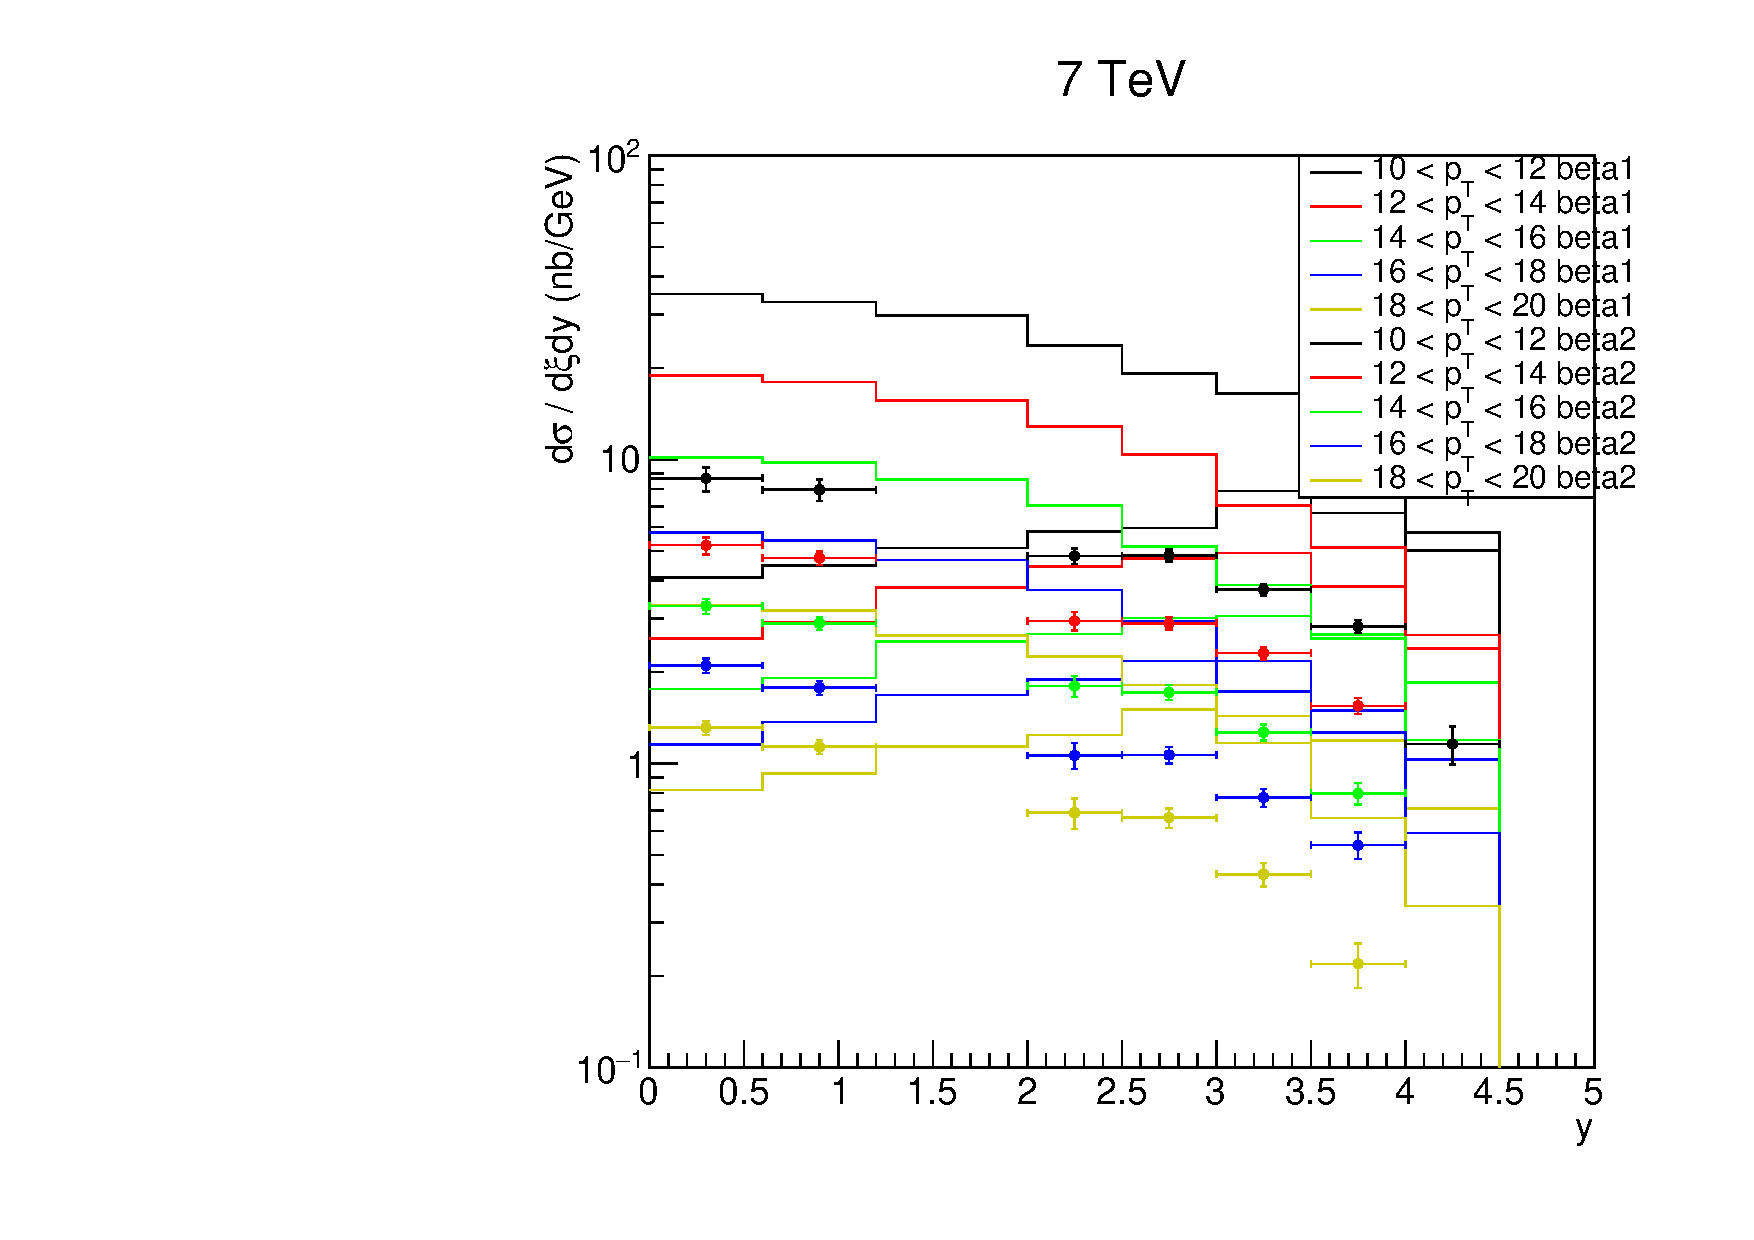
\includegraphics[width = 0.4\textwidth]{y_dist_log_7.pdf}
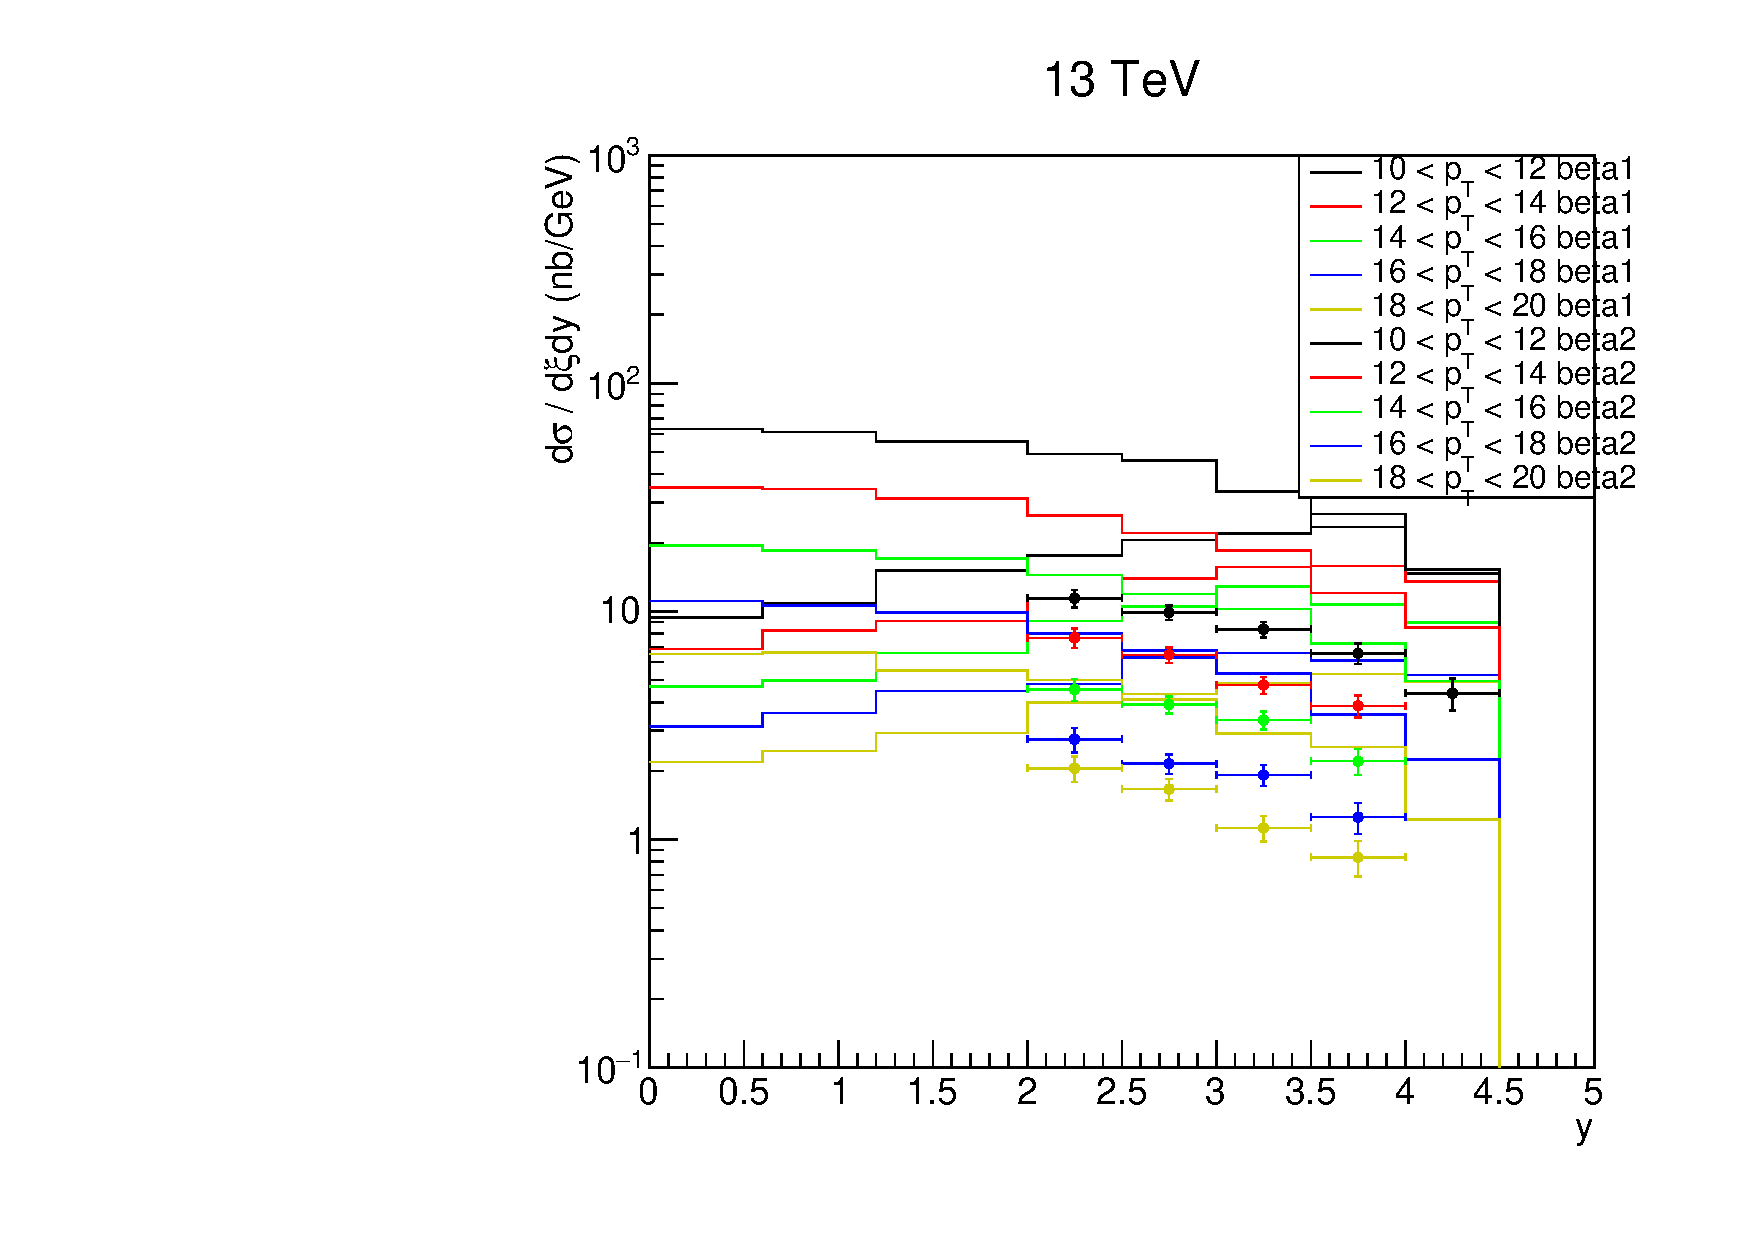
\includegraphics[width = 0.4\textwidth]{y_dist_log_13.pdf}
\caption{Comparison between MC $y$ distribution and data points in six  $\pt$ bins, for 7 TeV (left) and 13 TeV (right), in lin- (top) and log-scale (bottom). All histograms divided by total nr events and multiplied by same normalization factor. Data is not scaled.}\label{f:y_comp}
\end{figure}




\end{document}